\documentclass[tc, manuscript]{copernicus}

\usepackage{booktabs}
\usepackage{multirow}
\usepackage{siunitx} 

\begin{document}

\title{Fountain scheduling strategies for improving water-use efficiency of artificial ice reservoirs (Icestupas)}

\def\Authors{Suryanarayanan Balasubramanian\,$^{1,2}$, Martin Hoelzle\,$^{1}$Roger Waser\,$^{3}$}

\def\Address{$^{1}$University of Fribourg, Department of Geosciences, Fribourg, Switzerland $^{2}$University of
Applied Sciences and Arts, Luzern, Switzerland} \def\corrAuthor{Suryanarayanan Balasubramanian}
\Author[1,2]{Suryanarayanan}{Balasubramanian}
\Author[1]{Martin}{Hoelzle}
\Author[3]{Roger}{Waser}
\affil[1]{University of Fribourg, Department of Geosciences, Fribourg, Switzerland}
\affil[2]{Himalayan Institute of Alternatives, Ladakh, India}
\affil[3]{University of Applied Sciences and Arts, Luzern, Switzerland}

\correspondence{suryanarayanan.balasubramanian@unifr.ch}

\runningtitle{Scheduling AIR fountains}

\runningauthor{S. Balasubramanian}

\firstpage{1}

\maketitle

\begin{abstract}

  Artificial Ice Reservoirs (AIRs), often also called - Ice Stupas - are a climate change adaptation strategy
  developed in the Indian Himalayas (Ladakh). With this technology, otherwise unused stream water is stored in
  large ice towers in winter. The surplus melt water that is generated in spring is used for satisfying
  irrigation water demands. Recent studies have shown that during construction of traditional AIRs over 75 \% of
  the water sprayed was lost. Therefore, fountain wastewater production has to be reduced for improving water
  use efficiency.  During the winter of 2021-22, a traditional and an automated AIR were built in Guttannen,
  Canton of Berne, Switzerland with the main aim of comparing and quantifying the benefits of fountain
  scheduling. Fountain scheduling was realized through an automation system computing recommended discharge
  rates using real-time weather input and location metadata. The scheduled fountain produced similar volumes
  while consuming one-tenth of the water the unscheduled fountain used. Simulations converting unscheduled
  fountains to scheduled fountains improved the water use efficiency of several traditional AIRs more than two
  fold. Overall, these results show that the automated construction strategy can increase the water use
  efficiency of AIRs without compromising their meltwater production.

\end{abstract}

\introduction

Cryosphere-fed irrigation networks in arid mountain regions are completely dependent on timely availability of
meltwater from snow, glaciers and permafrost \citep{immerzeelImportanceVulnerabilityWorld2020, farhanHydrologicalRegimesConjunction2015,
tveitenGlacierGrowingLocal2007}. With the accelerated decline of glaciers due to climate change
\citep{nusserLocalKnowledgeGlobal2016}, cold arid mountain regions and their corresponding drainage system in the lowlands are experiencing water scarcity at certain places in the spring season like in Ladakh \citep{norphelSnowWaterHarvesting2015} or at other places in summer and early autumns seasons . This seasonal water scarcity makes it essential to provide
supplementary irrigation in order to sustain agricultural output and take advantage of the complete growing
season \citep{nusserLocalKnowledgeGlobal2016, vincentEnergyClimateChange2009}.

To cope with this recurrent water scarcity, villagers in the region of Ladakh have developed two types of
artificial ice reservoirs (AIRs): ice terraces and ice stupas (see Fig. \ref{fig:AIRforms}).  All these types of
ice reservoirs capture water in the autumn and winter, allowing it to freeze, and hold it until spring, when it
melts and flows down to fields \citep{ipccChapterHighMountain2019, vinceGlacierMan2009,
clouseLadakhArtificialGlaciers2017, nusserSociohydrologyArtificialGlaciers2019}. In this way, they retain a
previously unused portion of the annual flow and facilitate its use to supplement the decreased flow in the
following spring. This study focuses on the form of AIRs locally called as ice stupas.

\begin{figure}[t]
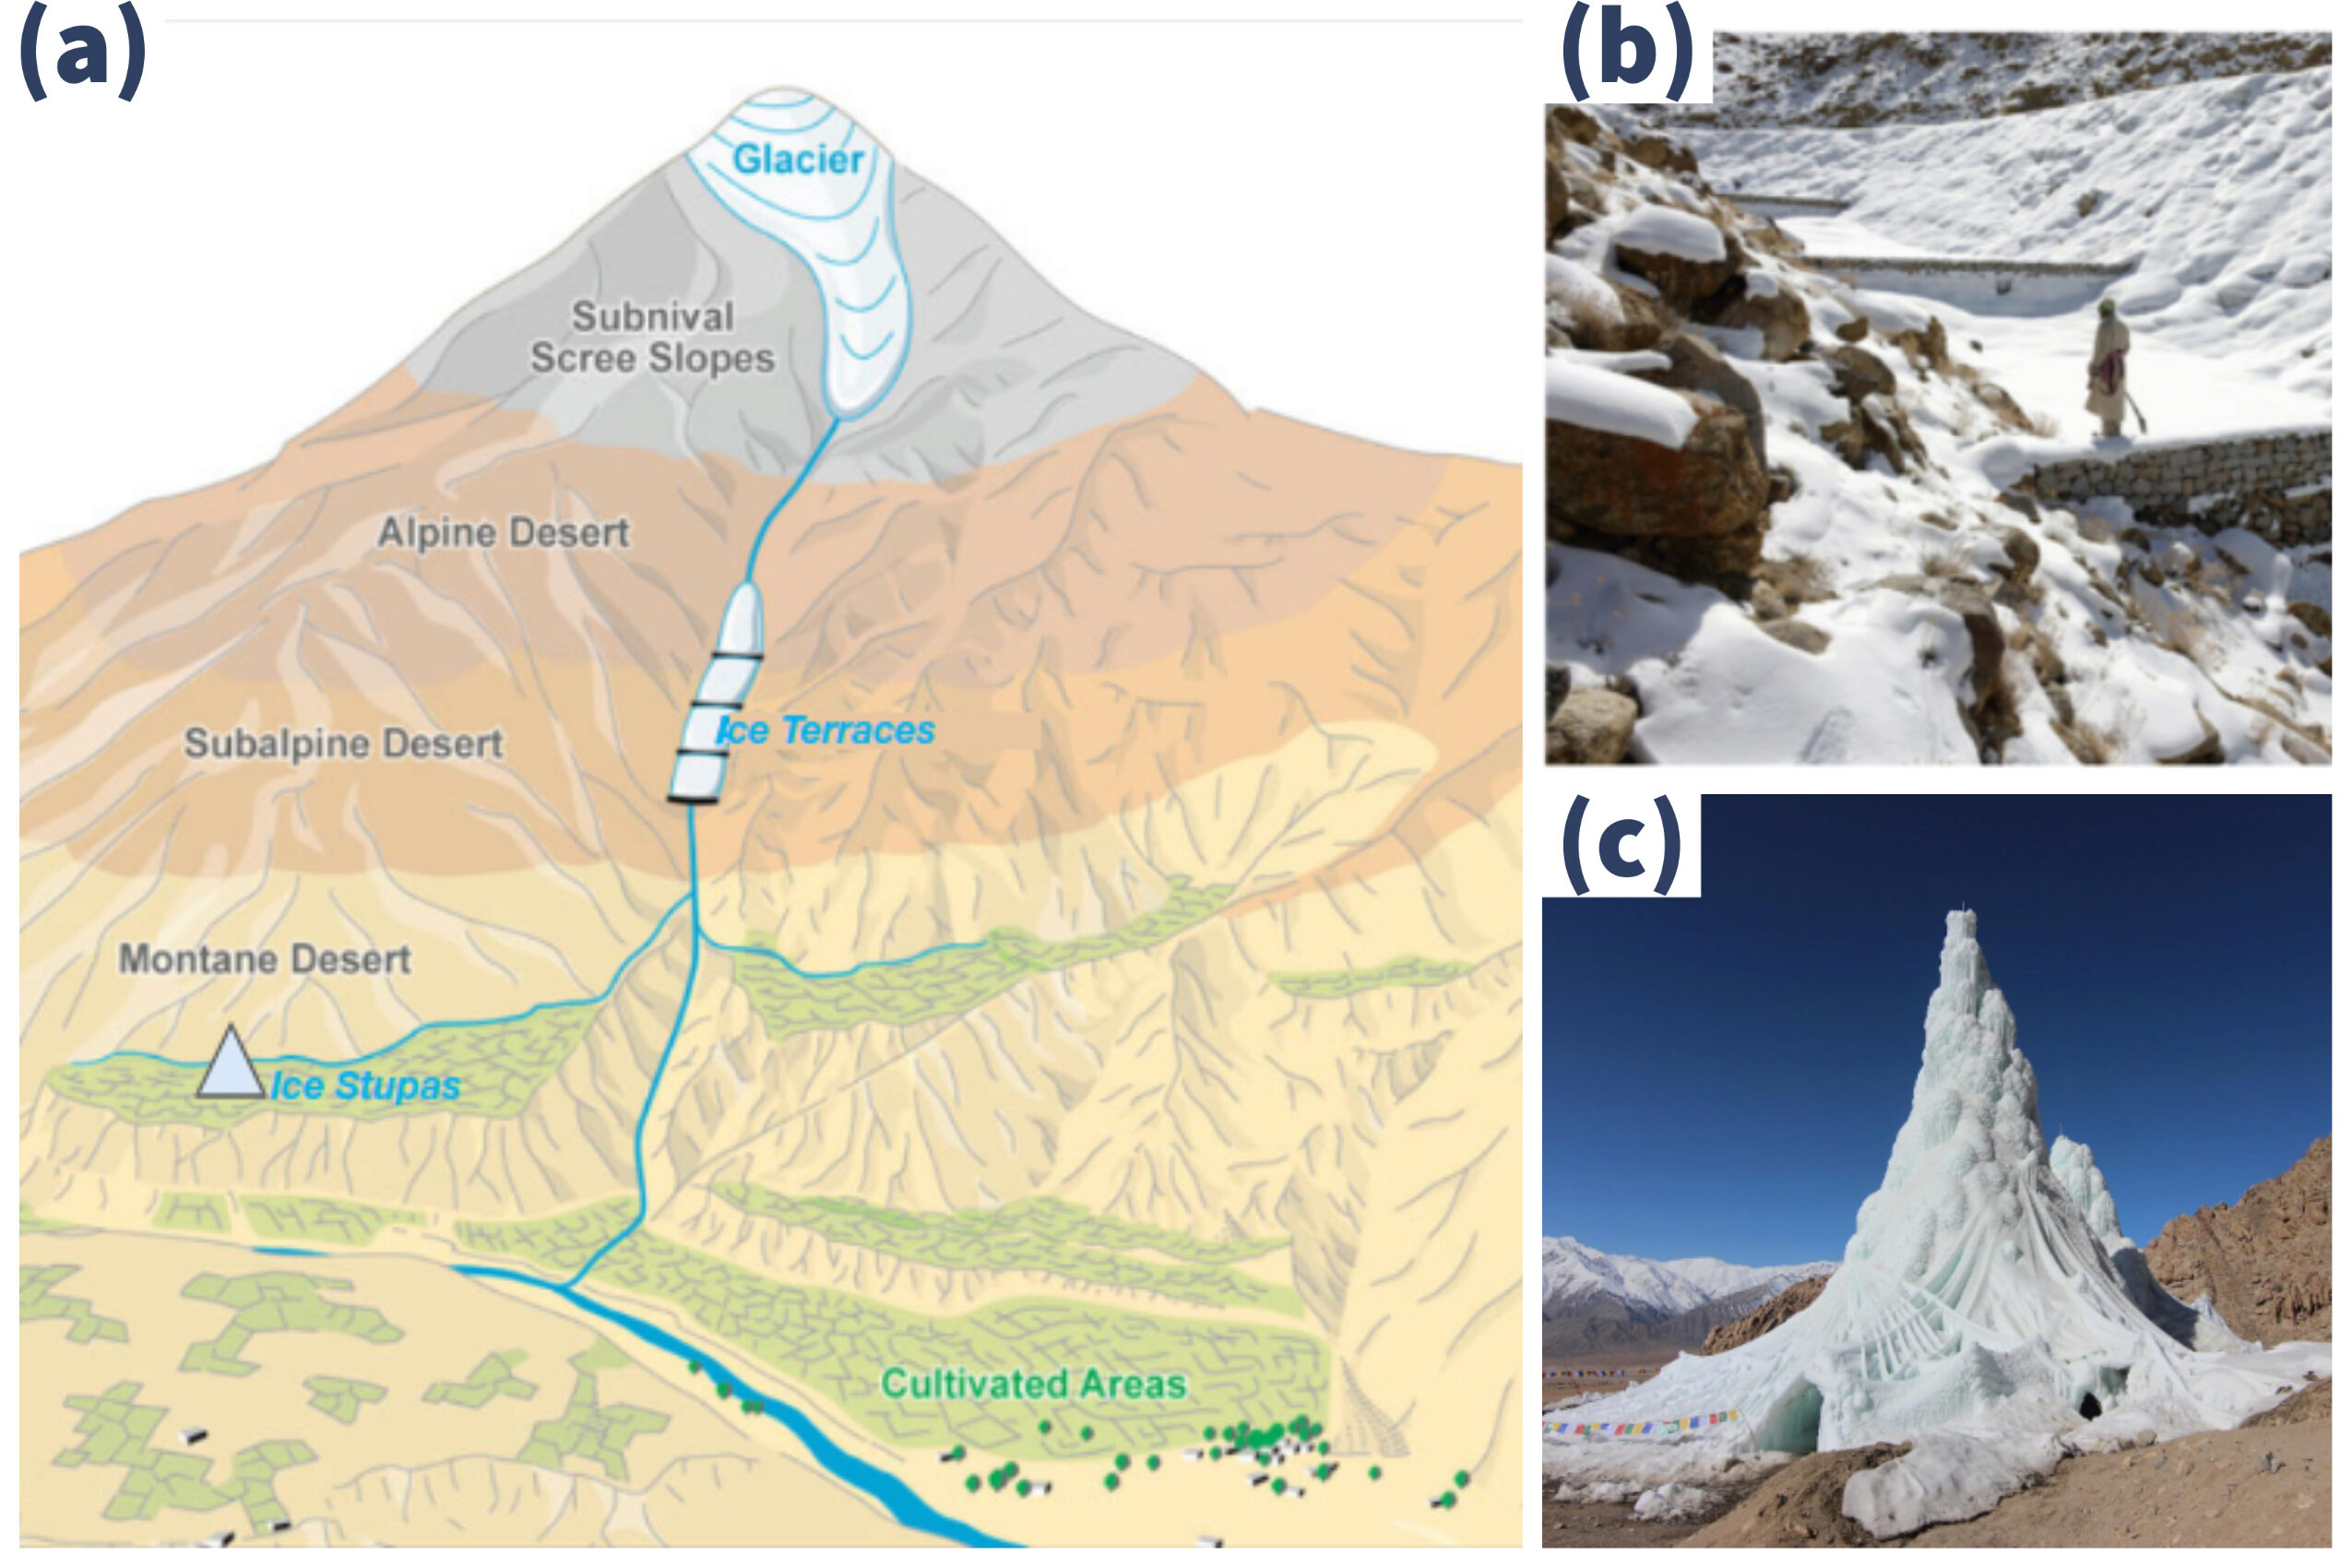
\includegraphics[width=12cm]{Figures/AIR_forms.jpg}

\caption{(a) Schematic overview of the position of artificial ice reservoirs. These constructions are located at
altitudes between the glaciers and the irrigation networks in the cultivated areas. Ice terraces and ice stupas
are located at higher and lower altitudes respectively. Adapted from: \cite{nusserLocalKnowledgeGlobal2016}}

\label{fig:AIRforms}
\end{figure}

Over the past decade, several ice stupas have been built to supplement irrigation water supply of mountain
villages in India \citep{wangchukIceStupaCompetition2020, palmerStoringFrozenWater2022,
aggarwalAdaptationClimateChange2021}, Kyrgyzstan \citep{bbcnewsBrightArtificialGlacier2020} and Chile
\citep{reutersConservationistsChileAim2021}. These AIRs are traditionally constructed by diverting springs or
glacial streams into fountain spray systems via embankments and pipelines. 

One of the common problems with AIR construction systems is related to fountain scheduling. Fountain scheduling
is simply answering the questions of “When do we spray?”, “How much do we spray?” and “How long do we spray?”.
Starting fountain spray too early or spraying too much water or running a fountain spray too long is considered
overwatering. At the very least this practice wastes water.  Likewise, starting fountain spray too late or
spraying too little water or not running the system for a long enough period of time is considered underwatering and can cause reduced ice volumes.

Previous work \citep{balasubramanianInfluenceMeteorologicalConditions2022} has shown that traditional
construction systems suffer from overwatering. In order to avoid this issue, it is important to understand surface freezing rates, which can be calculated by means of the full energy balance model
developed in \cite{balasubramanianInfluenceMeteorologicalConditions2022}. This model can be forced with either
historical weather data or real-time weather data to produce recommended discharge rates.

However, there are some practical issues that need to be addressed before dealing with the fountain scheduling
processes. For example, in the case of the Indian AIR, the fountain discharge rate could have been halved since
they were always two times higher than the modelled freezing rate
\citep{balasubramanianInfluenceMeteorologicalConditions2022}. However, in practice, reduction of discharge rate
would increase the maintenance cost due to higher risk of freezing events in the fountain pipeline.

An optimum construction strategy, therefore, should first prevent the occurrence of this event. These fountain
freezing events can be prevented by setting a minimum threshold for the recommended discharge rate.
Additionally, recommended discharge rate needs to be sensitive to constraints on the water supply or weather of
the construction site. Locations limited by their water supply like in Ladakh, India would prioritize water use
efficiency whereas those limited by the favourable weather windows like in Guttannen, Switzerland  would
prioritize for maximum ice volume.  Accordingly, we use two types of model parameter optimizations that prevent
underwatering and overwatering to attain higher ice volumes and higher water use efficiency respectively.

However, manually adjusting the fountain discharge rate is not practical due to two reasons. Firstly, this would
involve constant adjustments of discharge rates in response to the significant diurnal and seasonal variations
of the freezing rates. Secondly, frequent pipeline water drainage is required to avoid water losses. Therefore,
operation of scheduled fountains via automation systems is preferred to reduce the long-term maintenance costs.

The present study was performed to compare two AIRs produced using different fountain scheduling strategies but
exposed to identical meteorological conditions. The specific objectives of this study are to compare the
water-use efficiency, maximum ice volume and maintenance effort between the different fountain scheduling strategies.

\section{Study sites and data}

In this study, we use datasets presented in our previous work
\citep{balasubramanianInfluenceMeteorologicalConditions2022} along with new datasets. These old datasets record
the meteorological conditions and fountain characteristics of AIRs built in Gangles, India (IN21) and Guttannen,
Switzerland (CH21) during the winter of 2020-21. In this section, we focus on describing the new AIR datasets
collected in Guttannen, Switzerland during the winter of 2021-22 (CH22).

The Guttannen site (46.66 $\degree$N, 8.29 $\degree$E) is situated in the Berne region, Switzerland and has an
altitude of 1047 $m$ a.s.l. In the winter (Oct-Apr), mean daily minimum and maximum air temperatures vary
between -13 and 15 $\degree C$. Clear skies are rare, averaging around 7 days during winter. Daily winter
precipitation can sometimes be as high as 100 $mm$. These values are based on 30 years of hourly historical
weather data measurements \citep{meteoblueClimateGuttannen2021}. Two AIRs were constructed by the Guttannen
Bewegt Association, the University of Fribourg and the Lucerne University of Applied Sciences and Arts during
the winters of 2021-22 using a traditional and an automated construction strategy.

\begin{figure}[t]
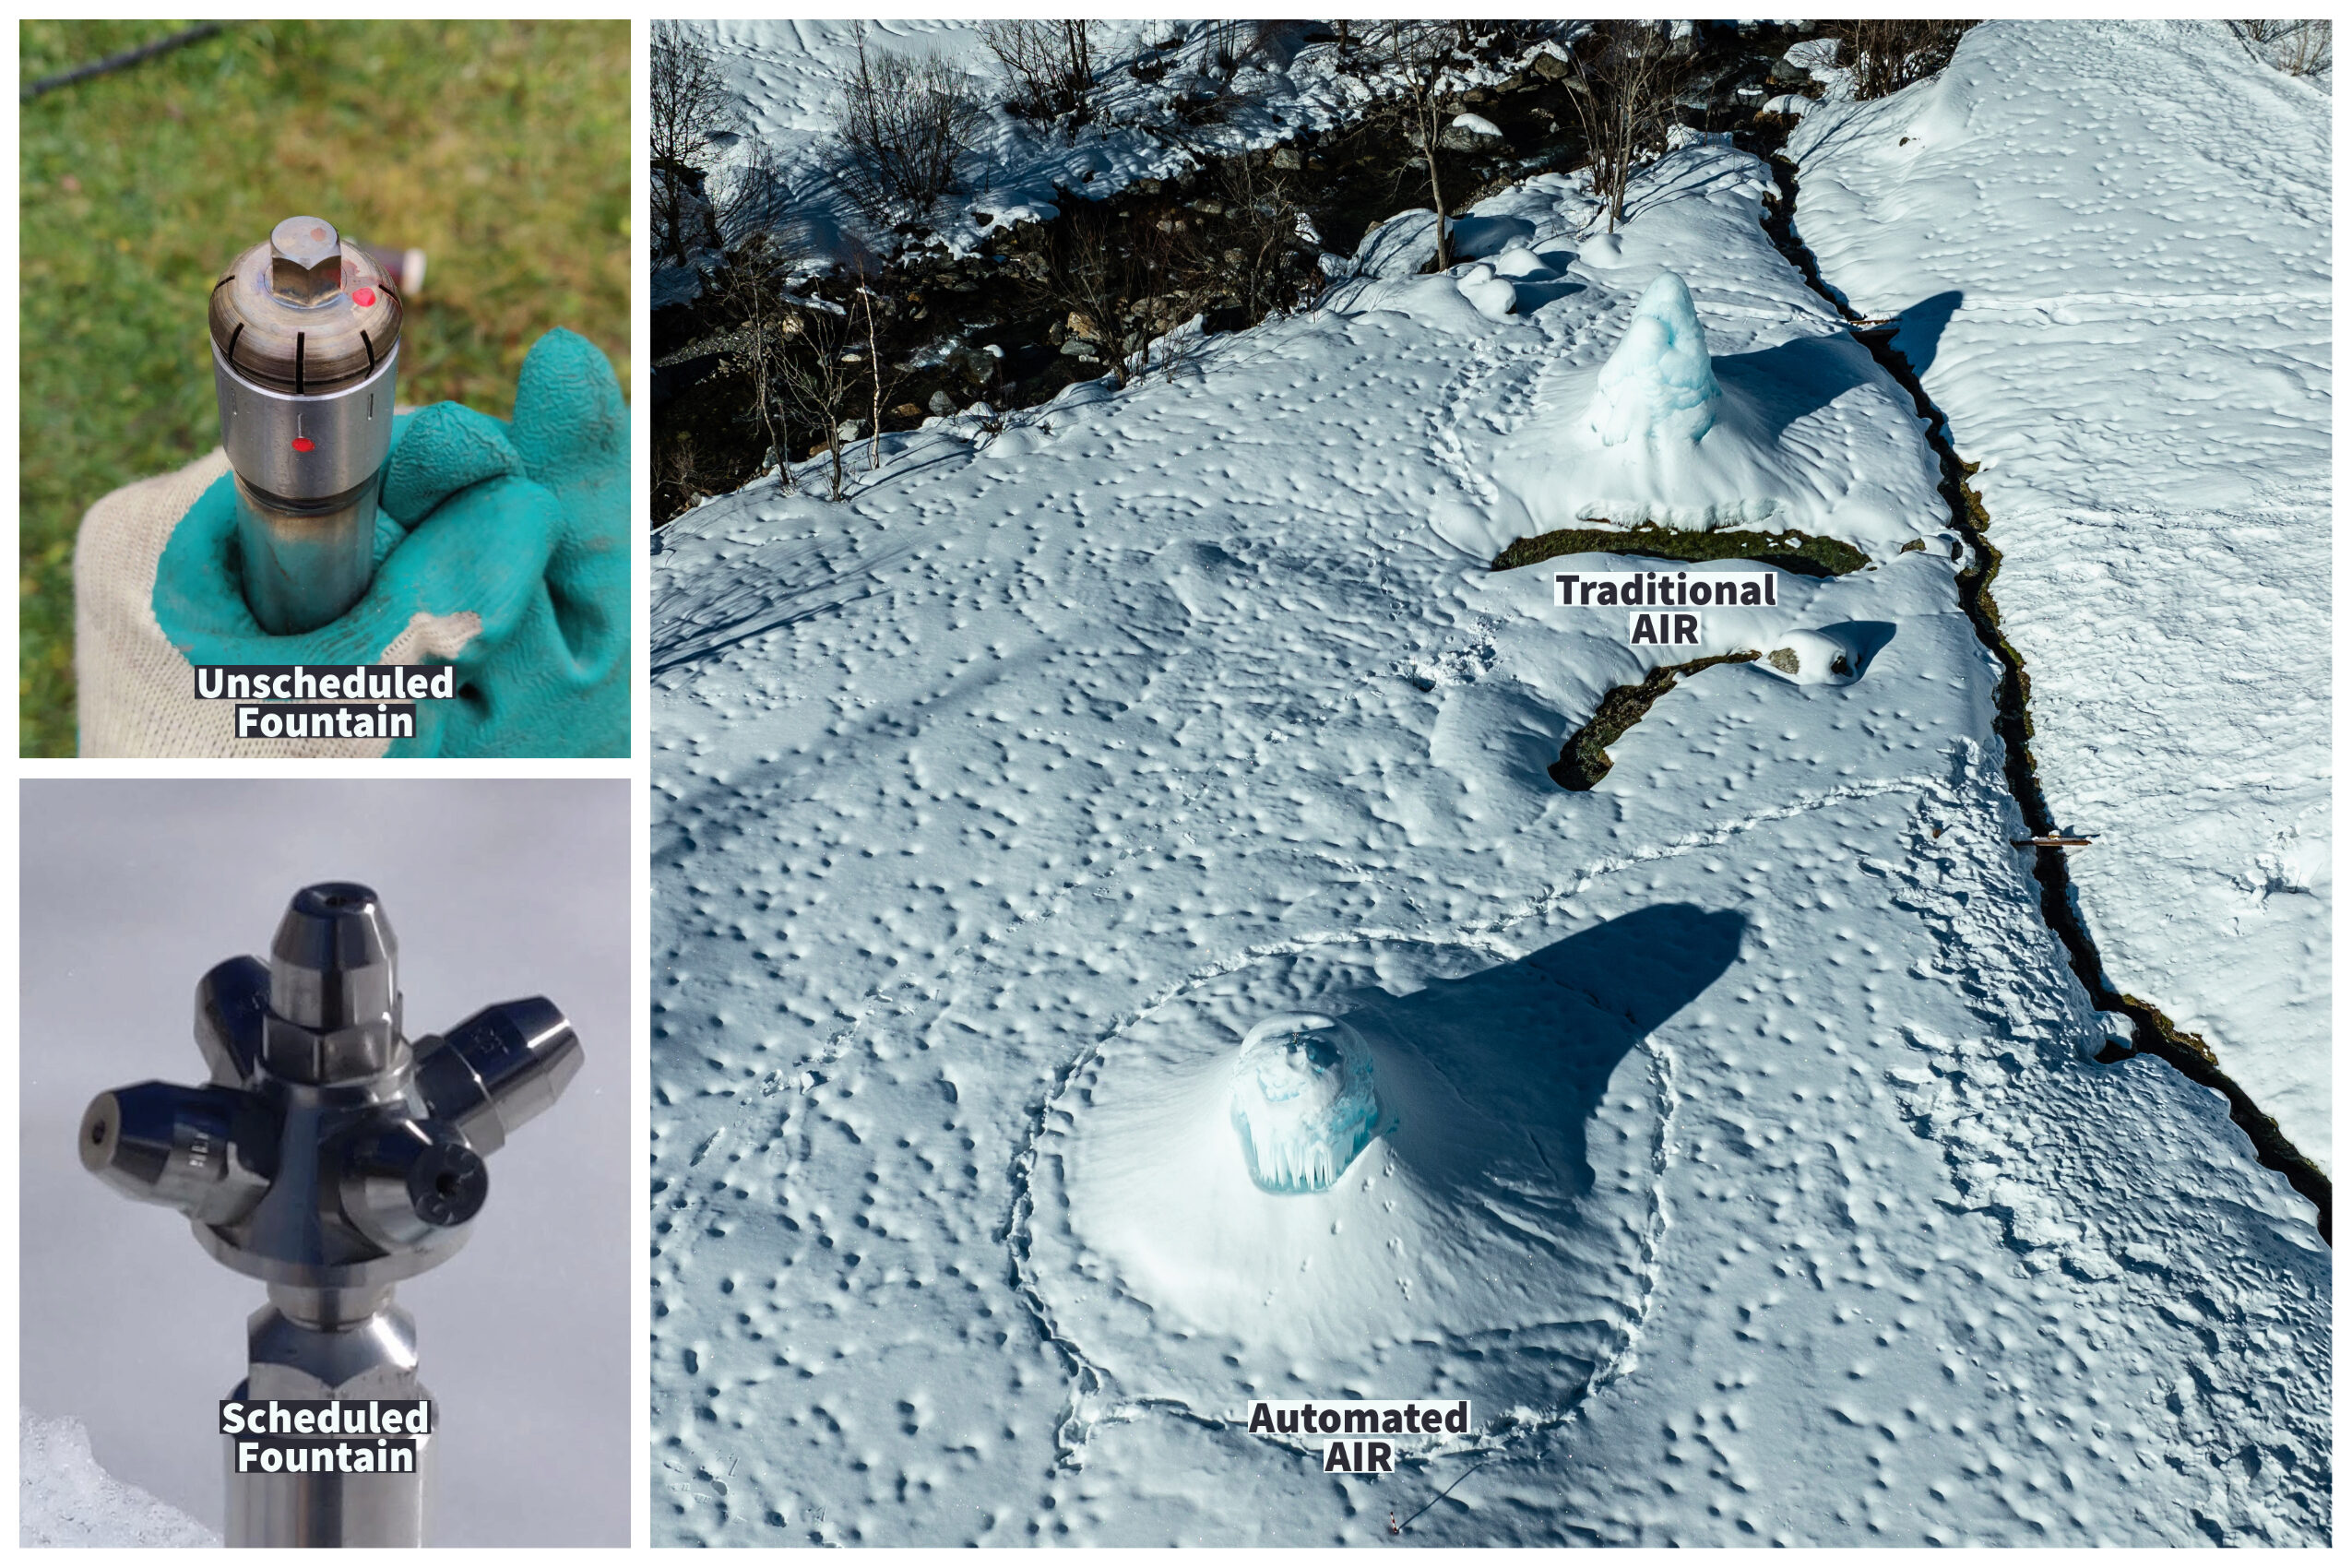
\includegraphics[width=12cm]{Figures/AIR_fountains.jpg}
\caption{Unscheduled and scheduled fountains used for construction of traditional an automated AIRs at Guttannen. Picture credits: Daniel Bürki}
\label{fig:2AIR}
\end{figure}

The automated and the traditional AIRs were constructed adjacent to each other but with different fountain
designs as shown in Fig. \ref{fig:2AIR}. This ensured both AIRs shared the same water source and identical
weather conditions. In addition, a webcam guaranteed a continuous survey of the automated AIR.   

In the traditional strategy, the fountain was operated manually whereas in the automated strategy a programmed
automation system controlled the fountain discharge rate during the whole study period using real time weather
input and several control parameters, which could be modified via a user interface. Henceforth, we refer to the
fountain used in the traditional and automated construction strategy as unscheduled and scheduled fountains,
respectively.

In the traditional construction strategy, tree branches were laid covering the fountain pipe to initiate and
speed up the ice cone formation process. In the automated strategy, only the fountain pipe was placed before the
water spray started. The construction of both the AIRs began on 8th December on a snow bed of 13 cm thickness
and ended on 12th April. These two dates are denoted as start and expiry dates henceforth.

\subsection{Meteorological data}

Air temperature, relative humidity, wind speed, pressure, precipitation, incoming long-wave radiation,
short-wave radiation and cloudiness index are required to calculate the surface energy balance of an AIR. The
primary weather data source was an automatic weather station (AWS) located around 20 m away. Hourly ground
temperature measurements were also recorded by the AWS to approximate the fountain's water temperature. Less
than 0.4 \% of the data was found to be missing and the data gaps were filled by linear interpolation. However,
two additional datasets were required to obtain all the necessary input variables, namely, cloudiness index and
precipitation. These two datasets were obtained from ERA5 reanalysis dataset
\citep{hersbachERA5GlobalReanalysis2020} and a MeteoSwiss AWS located 184 m away (Station ID: 0-0756-0-GTT)
respectively.

\begin{figure*}[t]
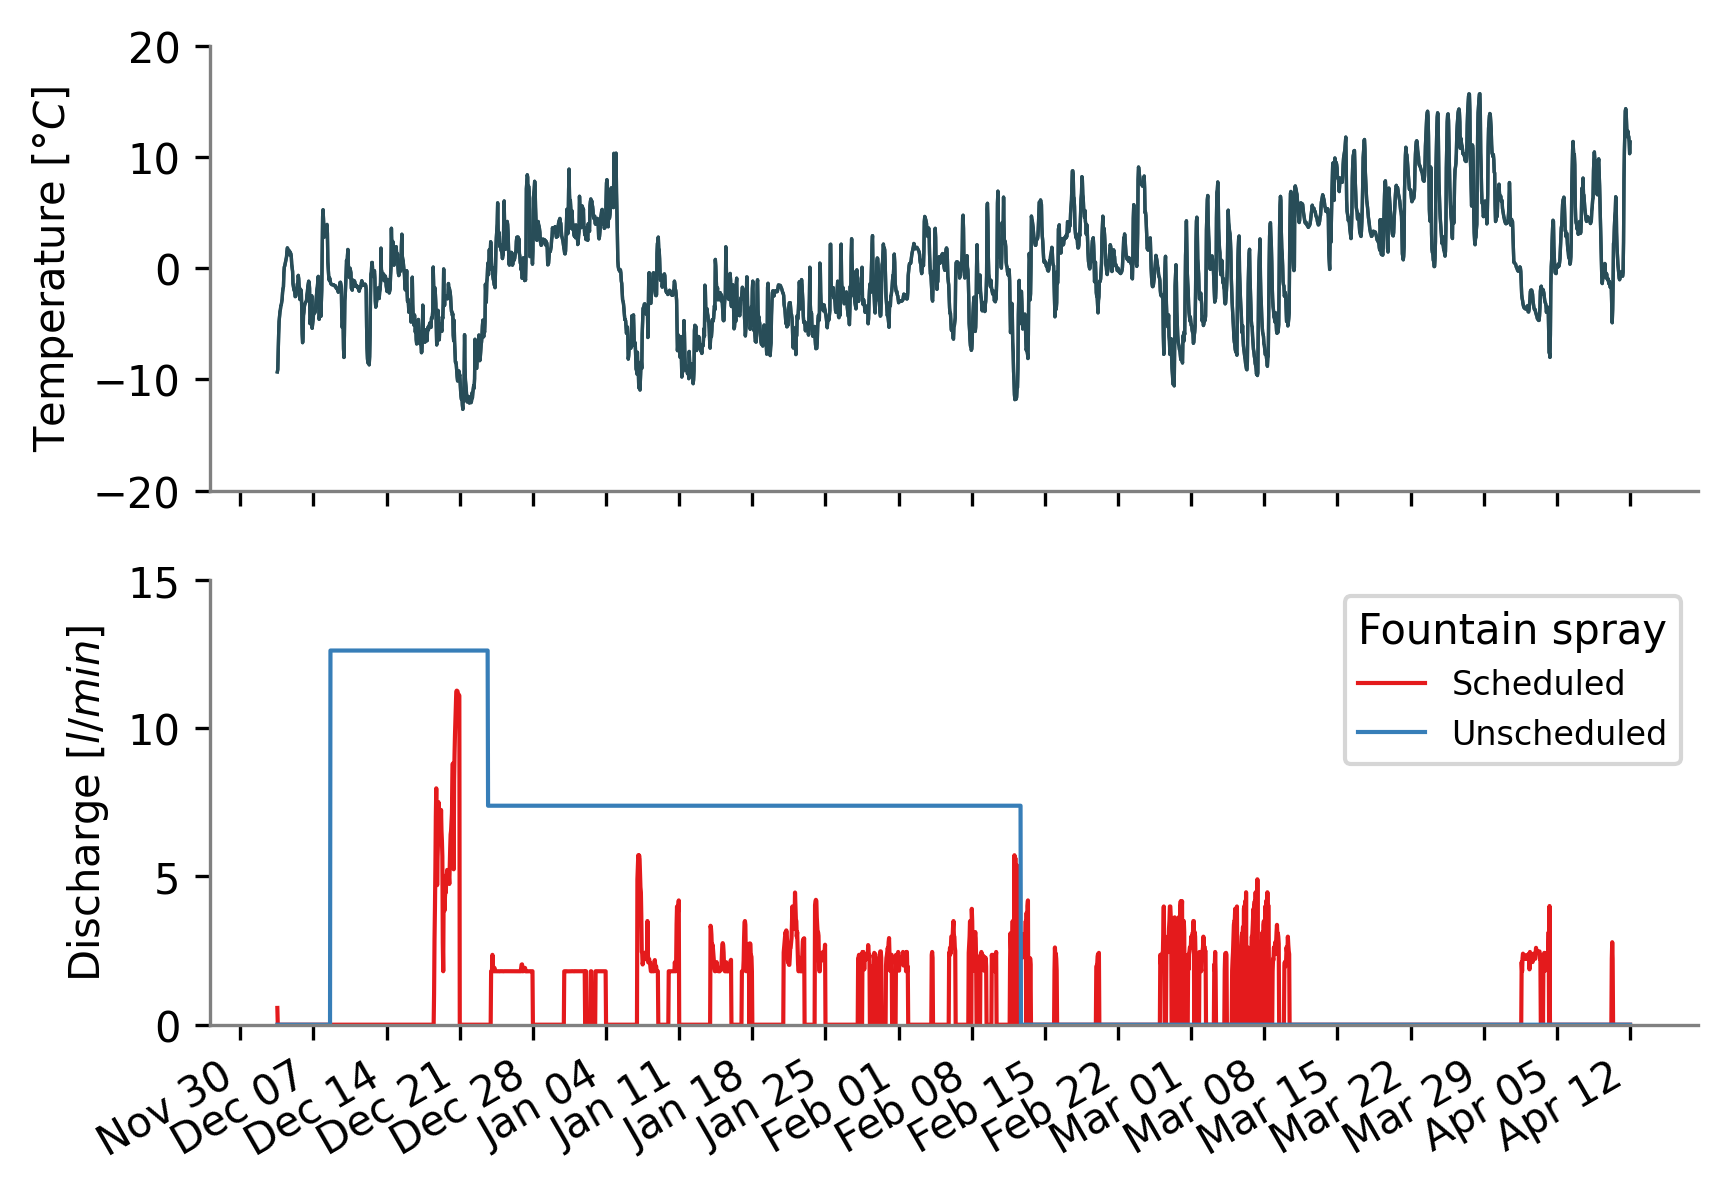
\includegraphics[width=12cm]{Figures/disvstemp.png}
\caption{Temperature and discharge measurements at the Guttannen construction site}
\label{fig:aws} 
\end{figure*}

\subsection{Fountain observations}

The scheduled and unscheduled fountains have four attributes, namely: discharge rate ($Q$), height ($h$), water
temperature ($T_F$), nozzle pressure loss ($P_{nozzle}$), and the spray radius ($r$). Discharge rate represents
the discharge rate of the water in the fountain pipeline. Height denotes the height of the fountain pipeline
installed. Fountain water temperature is the temperature of water droplets produced by the fountain. The nozzle
pressure loss denotes the preesure consumed during the formation of water droplets. Spray radius denotes the
observed ice radius formed from the fountain water droplets.

The height was increased in steps of 1 meter for both fountains. For the scheduled fountain, the
construction began with a height of 3 $m$ with an increase to 4 $m$ on 23rd December. For the unscheduled
fountain, the construction began with a height of 3.7 $m$ and was increased two times on 23rd December
and 12th February.

Fig. \ref{fig:aws} shows how the automation system operated the scheduled fountain based on real-time
meteorological conditions. The automation system caused these variations through its control valve which used
the recommended discharge rate to regulate the pipeline crosssectional area between 0 to 100 \% . Throughout the
study period, the control valve was opened completely (100 \%) only once corresponding to the time when the
temperature attained its minimum of -13 $\degree/,C$ on 20th December. After this event, the control valve was
never opened beyond 34 \% of the pipeline crosssectional area.  

The unscheduled fountain was manually operated to spray all the available discharge until a fountain freezing
event interrupted the discharge on 17th February. Unfortunately, no discharge rate measurements were recorded
for the unscheduled fountain. However, the unscheduled fountain was observed to have a higher discharge rate
compared to the scheduled fountain due to its higher aperture area (see Fig. \ref{fig:2AIR}). Therefore, we
conservatively assume the discharge rate of the unscheduled fountain to be equal to the maximum discharge rate
of the scheduled fountain which was observed to be 13 $l/min$ at a fountain height of 3 $m$ and 11 $l/min$ at a
fountain height of 4 $m$ respectively.

The water temperature of both the fountains were estimated from the AWS ground temperature dataset. This dataset
was acquired through a thermistor located 0.3 $m$ below the base of the fountain.

\subsection{Drone surveys}

Several photogrammetric surveys were conducted on the traditional and the automated AIRs. The details of these
surveys and the methodology used to produce the corresponding outputs are explained in
\cite{balasubramanianInfluenceMeteorologicalConditions2022}. The digital elevation models (DEMs) generated from
the obtained imagery were analysed to document the ice radius, the surface area and the volume of the ice
structures. Ice radius measurements of drone flights which observed either an increase in AIR circumference or
volume were averaged to determine the fountain's spray radius. The number of drone surveys conducted for the
traditional and the automated AIRs were 8 $m$ and 6 $m$, respectively (see Table \ref{tab:uav}). 

\begin{table}
	\centering
	\caption{Summary of the drone surveys}
	\label{tab:uav}
	\begin{tabular}{@{}|llllll|@{}}
		\toprule
		\textbf{}              & \textbf{No.} & \textbf{Date} & \textbf{Volume} & \textbf{Radius} & \textbf{Surface Area} \\ \midrule
		\multicolumn{1}{|l|}{\multirow{8}{*}{\rotatebox[origin=c]{90}{Traditional}}}
		                       & 1            & Dec 23, 2021  & 17 $m^{3}$     & 2.9 $m$
		                       & 47 $m^{2}$                                                                      \\
		\multicolumn{1}{|l|}{} & 2            & Jan 3, 2022  & 22 $m^{3}$     & 3.4 $m$
		                       & 61 $m^{2}$                                                                      \\
		\multicolumn{1}{|l|}{} & 3            & Jan 22, 2022   & 35 $m^{3}$     & 4 $m$
		                       & 79 $m^{2}$                                                                      \\
		\multicolumn{1}{|l|}{} & 4            & Feb 6, 2022  & 44 $m^{3}$     & 4.2 $m$
		                       & 86 $m^{2}$                                                                      \\
		\multicolumn{1}{|l|}{} & 5            & Feb 20, 2022  & 43 $m^{3}$     & 4.3 $m$
		                       & 86 $m^{2}$                                                                      \\
		\multicolumn{1}{|l|}{} & 6            & Mar 19, 2022  & 33 $m^{3}$     & 4.4 $m$
		                       & 84 $m^{2}$                                                                      \\
		\multicolumn{1}{|l|}{} & 7            & Mar 26, 2022  & 24 $m^{3}$     & 4.3 $m$
		                       & 74 $m^{2}$                                                                      \\
		\multicolumn{1}{|l|}{} & 8            & Apr 12, 2022  & 11 $m^{3}$     & 3.5 $m$
		                       & 50 $m^{2}$                                                                      
		\\\midrule
		\multicolumn{1}{|l|}{\multirow{6}{*}{\rotatebox[origin=c]{90}{Automated}}}
		                       & 1            & Dec 23, 2021  & 35 $m^{3}$      & 4.3 $m$
		                       & 73 $m^{2}$                                                                       \\
		\multicolumn{1}{|l|}{} & 2            & Jan 3, 2022   & 32 $m^{3}$      & 4.4 $m$
		                       & 81 $m^{2}$                                                                       \\
		\multicolumn{1}{|l|}{} & 3            & Feb 20, 2022   & 60 $m^{3}$      & 5.3 $m$
		                       & 105 $m^{2}$                                                                       \\
		\multicolumn{1}{|l|}{} & 4            & Mar 19, 2022   & 28 $m^{3}$      & 3.7 $m$
		                       & 57 $m^{2}$                                                                       \\
		\multicolumn{1}{|l|}{} & 5            & Mar 26, 2022   & 19 $m^{3}$      & 3.7 $m$
		                       & 53 $m^{2}$                                                                       \\
		\multicolumn{1}{|l|}{} & 6            & Apr 12, 2022   & 7 $m^{3}$      & 2.5 $m$
		                       & 53 $m^{2}$                                                                       \\
		\bottomrule
	\end{tabular}

\end{table}

\section{Methods}

\subsection{Discharge scheduling software}

The software used for fountain scheduling was obtained by extending the AIR model developed in
\citep{balasubramanianInfluenceMeteorologicalConditions2022}. This software recommended two types of fountain
scheduling strategies based on the requirements of the construction location. The software recommended
water-sensitive fountain scheduling strategies if the location had limited quantity of water whereas
weather-sensitive fountain scheduling strategies if the location had limited duration of favourable weather
windows. These two kinds of scheduled fountains will be referred to as water-sensitive fountain and
weather-sensitive fountain henceforth.

Water-sensitive fountains are expected to produce higher water use efficiency whereas weather-sensitive fountains
are expected to produce higher ice volumes. Accordingly, we produce the discharge rate recommendations for these
two kinds of fountains through two sets of model forcing assumptions for the following three model variables:
(a) slope , (b) albedo and (c) cloudiness.  These two kinds of models will be referred to as ice volume
optimised model (IVOM) and water-use efficiency optimised model (WEOM), respectively. The slope variable
increases the shortwave radiation and sensible heat impact. The albedo variable decreases the shortwave
radiation impact. The cloudiness variable increases both the shortwave and the longwave radiation impact. We
associate the upper and lower bounds of these variables with the IVOM and WEOM versions depending on whether
they overestimate and underestimate the freezing rate of the AIR as shown in Table \ref{tab:assumptions}.

\begin{table}[]
\centering
\caption{Assumptions for the parametrisation introduced to simplify the ice volume optimised model (IVOM) and
water-use efficiency optimised model (WEOM).}
\label{tab:assumptions}
\begin{tabular}{@{}lllll@{}}
\toprule
\textbf{Estimation of} & \textbf{Symbol} & \textbf{IVOM} & \textbf{WEOM} & \\ \midrule
\multicolumn{1}{|l}{Slope}        & $s_{cone}$ & $ 1 $ & $0$ & \multicolumn{1}{l|}{} \\ \midrule
\multicolumn{1}{|l}{Albedo} & $\alpha$ & $\alpha_{snow}$ & $\alpha_{ice}$ & \multicolumn{1}{l|}{} \\\midrule 
\multicolumn{1}{|l}{Cloudiness}  & $cld$ & $0$ & $1$ & \multicolumn{1}{l|}{} \\ \bottomrule
\end{tabular}
\end{table}

We apply the assumptions described in Table \ref{tab:assumptions} on the one-dimensional description of energy
fluxes as used in \cite{balasubramanianInfluenceMeteorologicalConditions2022} to obtain the rate of change of
AIR ice mass as follows: 

\begin{equation}
  \frac{\Delta M_{ice}}{\Delta t}  =  (\frac{q_{SW} + q_{LW} + q_{S} + q_{F} + q_{R} + q_{G} - q_{T}}{L_F} + \frac{q_{L}}{L_V} ) \cdot A_{cone}
	\label{eqn:auto}
\end{equation}

Upward and downward fluxes relative to the ice surface are positive and negative, respectively. The first term
represents the mass change rate due to freezing of the fountain water and melting of the ice. $q_{SW}$ is the
net short-wave radiation; $q_{LW}$ is the net long-wave radiation; $q_{L}$ and $q_{S}$ are the turbulent latent
and sensible heat fluxes; $q_{F}$ is the fountain discharge heat flux; $q_{R}$ is the rain water heat flux;
$q_{G}$ is the ground heat flux; $q_{T}$ is the temperature heat flux and $A_{cone}$ is the area of the AIR
surface. The derivation of these individual terms for the IVOM and WEOM model versions are discussed in 
Appendix \ref{sec:SEB}.

Equation \ref{eqn:auto} is implemented in the automation system through a user interface that enables input of
the spray radius, altitude, latitude and longitude of the construction location. Once switched on, the
automation system regulates the fountain discharge rate based on the recommended discharge rate.

The automation hardware consists of an AWS, flowmeter, control valve, drain valves, air valves, fountain,
pipeline and a logger. The logger feeds the AWS data to the automation software and informs the recommended
discharge rate to the flowmeter. The flowmeter adjusts the control valve to match the recommendation. In case a
termination criteria is valid, the drain and air valves allow the removal of water from the pipeline and entry
of air in the pipeline respectively.

The recommended discharge rate is equal to the ice mass change rate. However, certain termination criteria
override the discharge rate recommendation and drain the pipeline to prevent water loss or fountain freezing
events, namely: 

\begin{itemize}

\item High water loss is assumed if wind speed is greater than the user-defined critical wind speed.

\item High risk of fountain freezing event is assumed if $\frac{\Delta M_{ice}}{\Delta t}$ is lower than the user-defined minimum fountain discharge rate. 

\item Freezing events in the fountain pipeline are assumed if measured discharge rate is zero for at least 20 seconds and the pipeline is drained as a
  consequence.

\item Pipeline leakage is assumed if measured discharge rate is greater than the user-defined maximum fountain discharge rate.

\end{itemize}

\section{Determination of pressure losses} \label{sec:p_loss}

The fountain pipeline system delivering water to the ice stupa suffers from several pressure losses. These
losses limit the maximum height that the fountain can achieve. There are three kinds of losses namely, (a)
altitudinal ($P_{alt}$), (b) frictional ($P_{friction}$) and (c) nozzle ($P_{nozzle}$) losses. The altitudinal
losses depend on the altitude difference between the source and the fountain. The frictional losses are
proportional to the length of the pipeline and inversely proportional to their diameter. The nozzle losses
depend on the engineering design of the fountain nozzle.

The pressure losses can be determined using the Bernoulli equation as follows:

\begin{equation}
  \label{eqn:pressure}
  P_{source} = P_{alt} + P_{friction} + P_{nozzle} + \frac{\rho \cdot v^2}{2}
\end{equation}

where $P_{source}$ is the source pressure , $P_{nozzle}$ is the pressure loss due to the fountain nozzle and
$P_{alt}$ is pressure loss due to the altitudinal difference between the pipeline input and fountain
output. The velocity $v$ can be determined from discharge rate observations using Eqn. \ref{eqn:dis}. 

The frictional loss of the pipeline can be determined from the following equation taken from \ref{}:  

\begin{equation}
  \label{eqn:friction}
  P_{friction} = [4 \cdot 10 ^{-5} \cdot Q + 0.0002 \cdot Q] \cdot L
\end{equation}

where $L$ is the total length of the pipeline in $m$ and $Q$ is the discharge rate in $l/min$.


\subsection{Model updates}

In this article, we refrain from a more general model description and focus only on the
description of the integration of fountain scheduling processes. For details on the model internals, and the
calculation of surface processes we refer to the respective literature references. 

In the previous version of the model \citep{balasubramanianInfluenceMeteorologicalConditions2022}, the fountain
water temperature ($T_F$) was estimated as a constant parameter. However, in reality, this is a poor
approximation as it is not accounting for two processes, namely, (a) temperature fluctuations during transit
from the source to the fountain nozzle; (b) temperature fluctuations during the flight time of the water
droplets after leaving the fountain nozzle. Therefore, we instead use measured hourly ground temperature
measurements to approximate process (a) and assume water temperature cools down to 0 $\degree\,C$ during subzero
air temperature conditions to approximate process (b).

In the previous version of the model \citep{balasubramanianInfluenceMeteorologicalConditions2022}, fountain
discharge events were reset from surface albedo to ice albedo. However, this assumption limits the accuracy of
the model, especially, for the automated AIR, where several fountain discharge events of short duration occur.
Therefore, we assumed that discharge events instead reduce the albedo decay rate ($\tau$) by a 
factor of $\frac{\alpha_{ice}}{\alpha_{snow}}$.

Additionally, both the AIRs experienced many precipitation events. Therefore, it was no longer accurate to
assume AIR density ($\rho_{cone}$) to be equal to ice density. We instead parameterised AIR density $\rho_{cone}$ as follows:

\begin{equation}
  \rho_{cone} = \frac{M_{F} + M_{dep} + M_{ppt}}{(M_{F} + M_{dep})/\rho_{ice} + M_{ppt}/\rho_{snow}}
\end{equation}

where $M_F$ is the cumulative mass of the fountain discharge; $M_{ppt}$ is the cumulative precipitation;
$M_{dep}$ is the cumulative accumulation through water vapour deposition; $\rho_{ice}$ is the ice density (917
$kg\,m^{-3}$) and $\rho_{snow}$ is the density of wet snow (300 $kg\,m^{-3}$) taken from
\cite{cuffeyPhysicsGlaciers2010} .

Rain events were not considered in the previous version of the model but they occurred in our experiment. The
influence of rain events on the albedo and the energy balance was assumed to be similar to discharge
events. However, the water temperature of a rain event was assumed to be equal to the air temperature.
Accordingly, the heat flux generated due to a rain event was equal to:

\begin{equation}
  q_{R} = \frac{\Delta M_{ppt} \cdot c_{water} \cdot T_{a}}{\Delta t \cdot A_{cone}}
\end{equation}

\subsection{Calibration and Validation}

The model parameters were calibrated to the median values of the ranges presented in Appendix Table
\ref{tab:parameters}. However, the surface layer thickness parameter was calibrated to a value of 0.09 $m$ for the
automated AIR instead of the default value of 0.05 $m$. This calibration was necessary to prevent hourly surface
temperature fluctuations to assume unphysical values above 40 $\degree\,C$.

We performed the validation of the model on the traditional and automated AIRs by evaluating the root mean
squared error (RMSE) between volume estimates and measurements. 

The performance of the IVOM and WEOM versions of the physical model was assessed by comparing correlation of its
discharge rate estimates with the validated freezing rate of the traditional AIR.

\section{Results}

\subsection{Scheduled discharge rate simulations}

The water-sensitive and weather-sensitive fountains scheduled by the WEOM and IVOM model versions estimated the
freezing rate of the unscheduled fountain with a correlation of 0.4 and a RMSE less than 0.8 $l/min$ and 1.8
$l/min$, respectively. The weather-sensitive fountain overestimated the freezing rate 93 \% of the fountain spray
duration whereas the water-sensitive fountain overestimated the freezing rate 70 \% of the unscheduled fountain
spray duration as illustrated by Fig. \ref{fig:simvsreal}. Therefore, the IVOM model forcing was successful in
prioritizing the maximum ice volume but the WEOM model forcing could not optimize for water use efficiency.
However, this large overestimation could be due to the depression of the unscheduled fountain's freezing rate
caused by its excess discharge rate. 

\begin{figure*}[t]
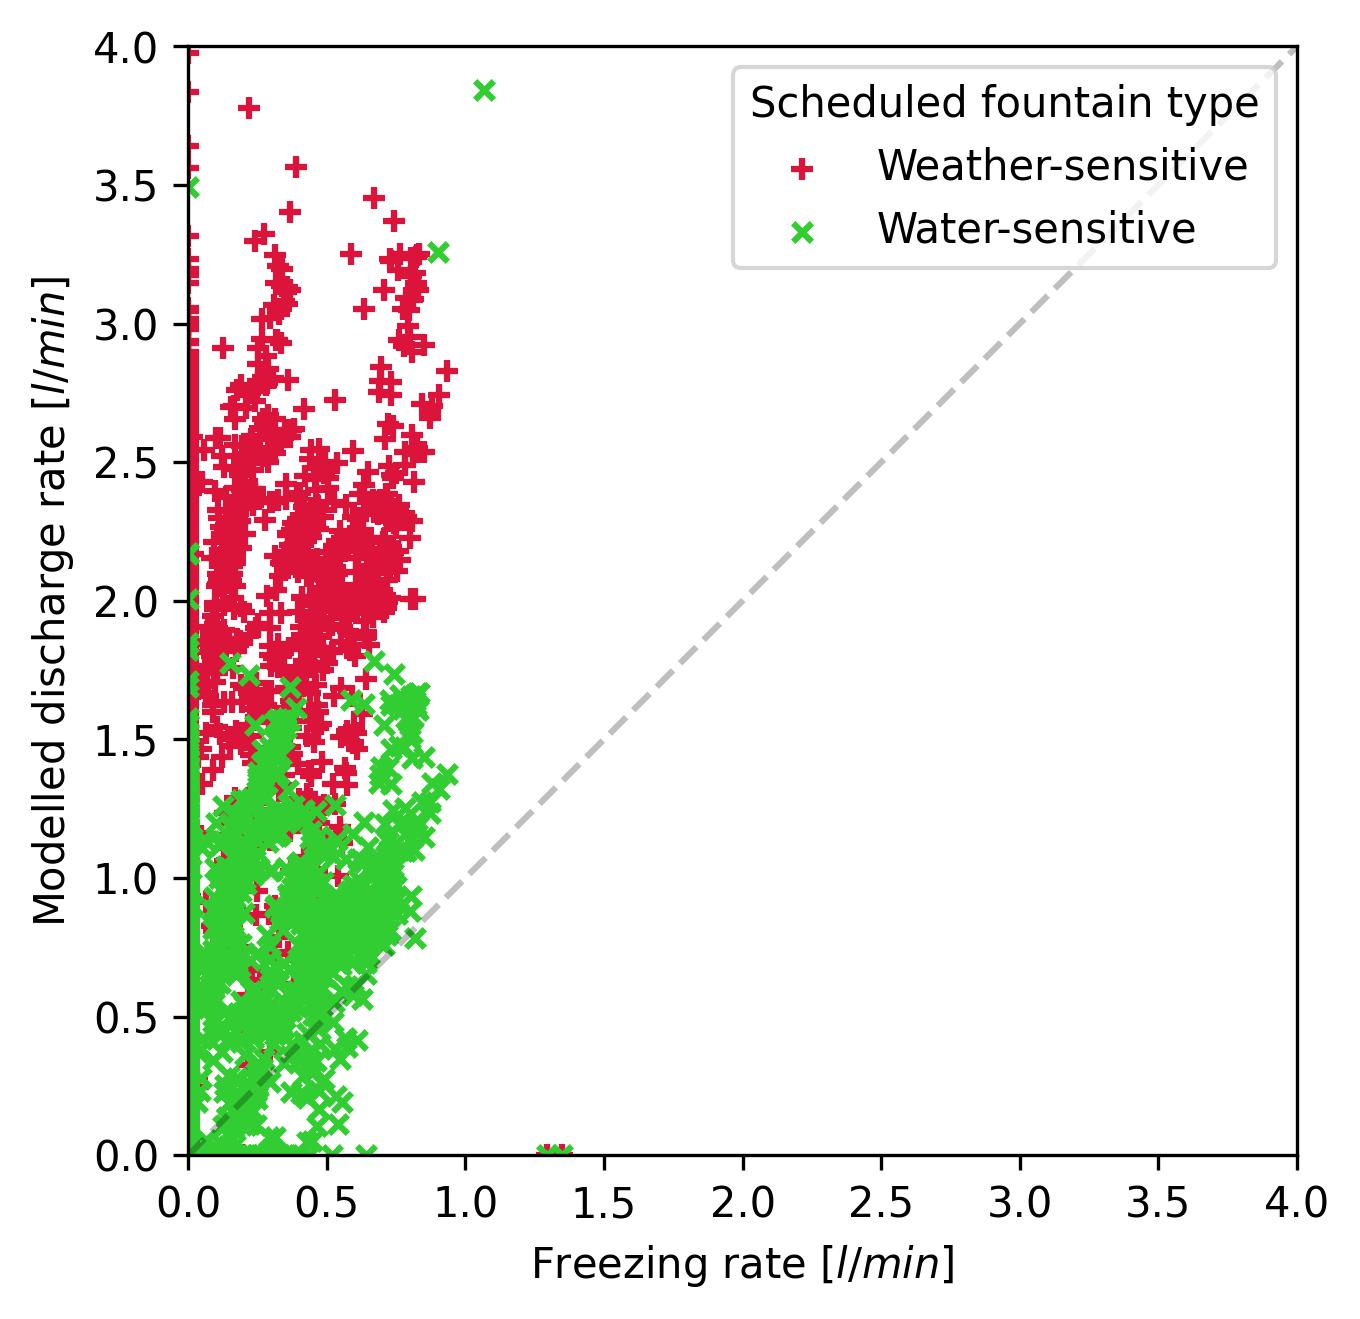
\includegraphics[width=8cm]{Figures/simvsreal.jpg}

\caption{ Comparison of the freezing rate estimated for the unscheduled fountain and the discharge rate of the
scheduled fountains. }

\label{fig:simvsreal}
\end{figure*}

\subsection{Model validation}

The volume estimation for the automated and traditional AIR had an RMSE of 8 $m^3$ and 6 $m^3$ with the drone
volume observations, respectively. This RMSE error is within 13 \% and 11 \% of the maximum volume of the
automated and the traditional AIR respectively. The estimated and measured AIR volumes are shown in Fig.
\ref{fig:validation}.  

\begin{figure*}[t] 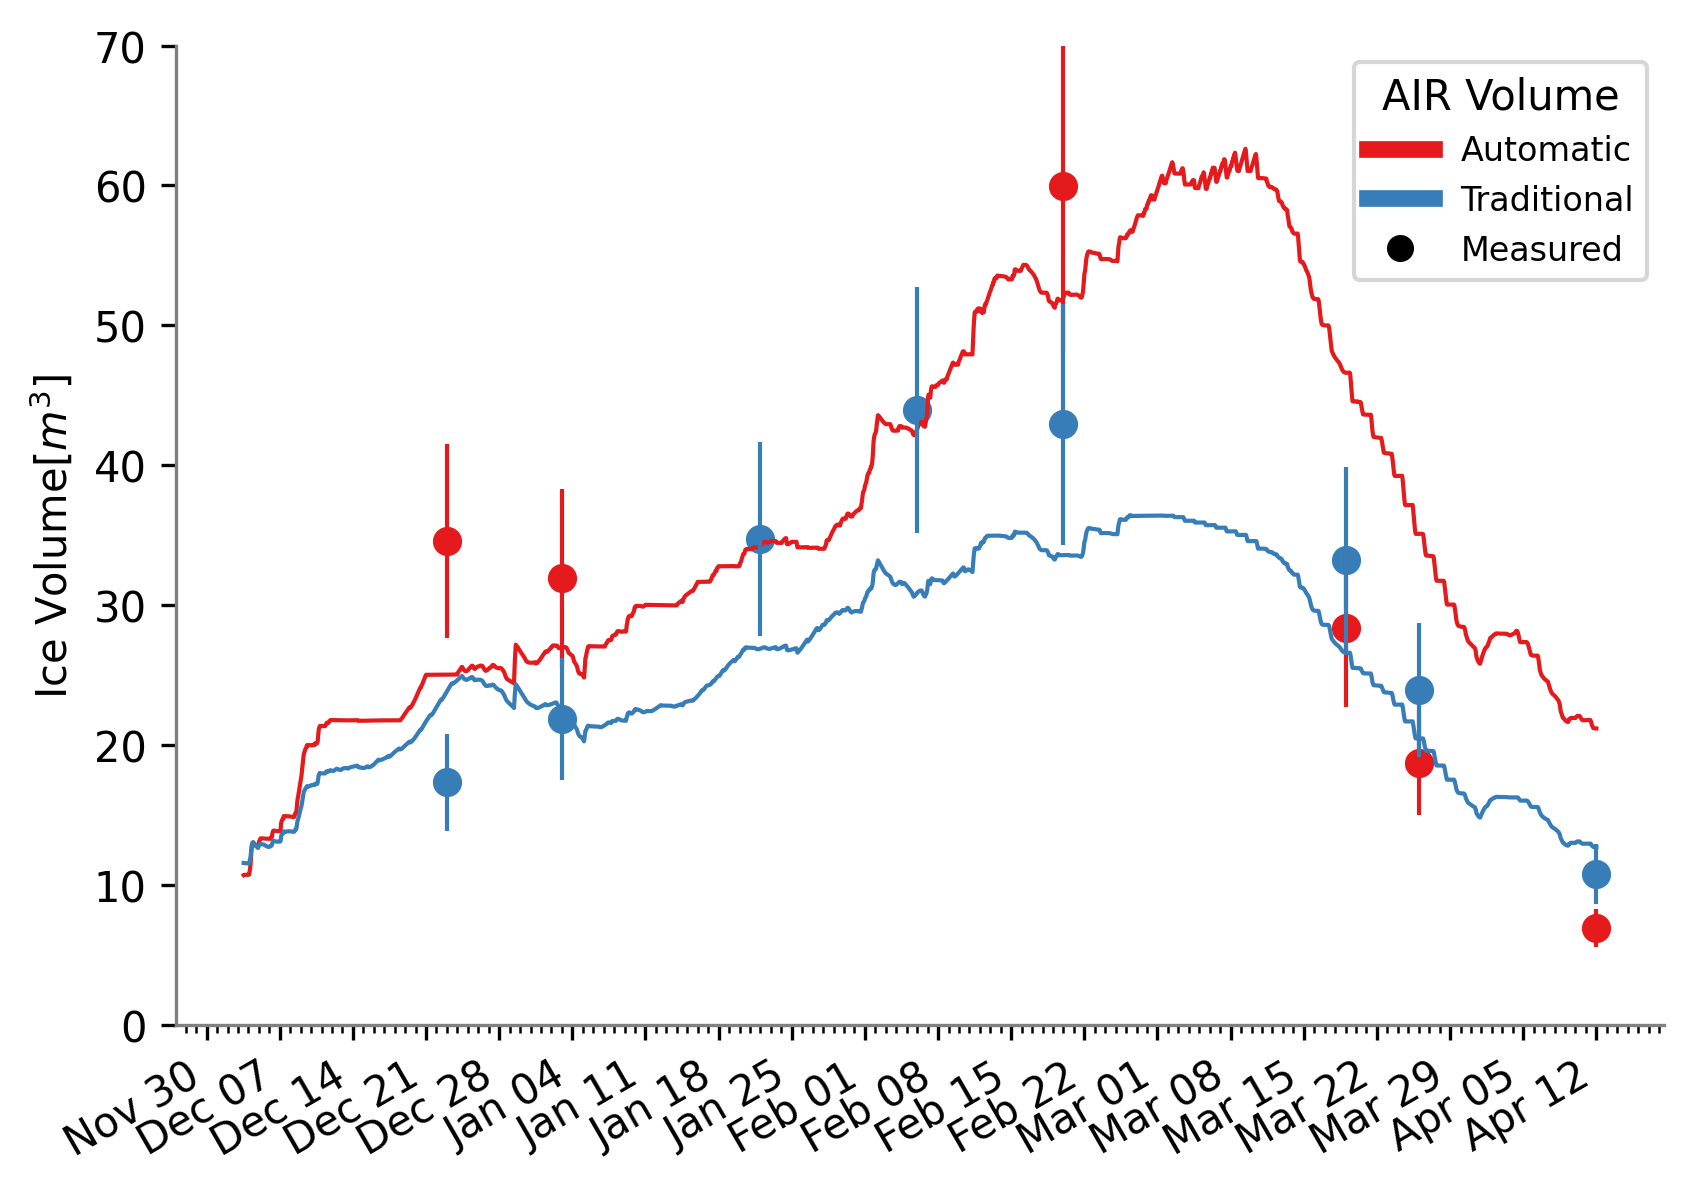
\includegraphics[width=12cm] {Figures/validation.png} \caption{Volume validation of the
scheduled and unscheduled fountain construction strategies.} \label{fig:validation} \end{figure*}

\begin{figure*}[t]
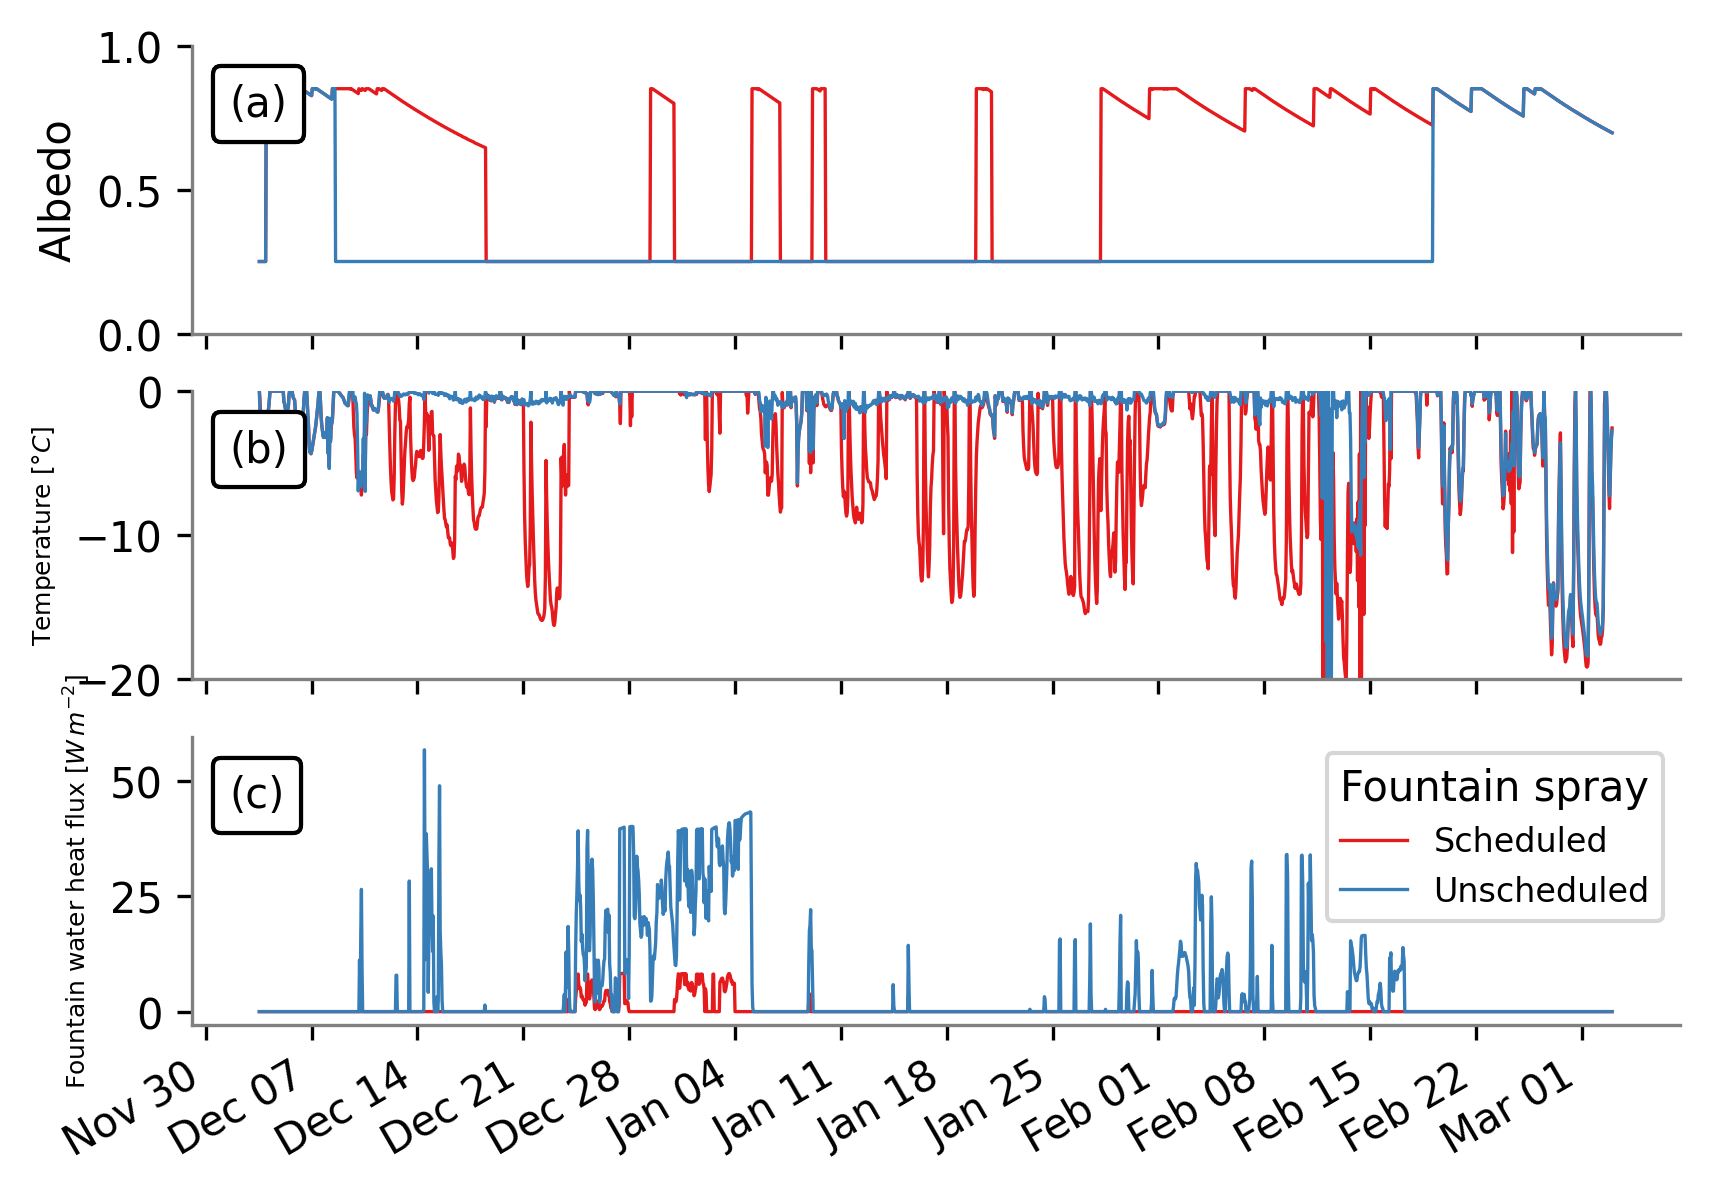
\includegraphics[width=12cm]{Figures/dis_processes.png}
\caption{(a) Surface albedo  and (b) fountain discharge heat flux showed significant variations between the two
  AIRS due to the differences in their discharge rates.}
\label{fig:dis_processes}
\end{figure*}

\begin{table}
	\centering
	\caption{Summary of the mass balance, energy balance, fountain and AIR characteristics estimated at the end of the respective
  simulation duration for the automated and the traditional AIRs}
	\label{tab:mb}
	\begin{tabular}{@{}|llllll|@{}}
		\toprule
		\textbf{}              & \textbf{Name}                   & \textbf{Symbol} & \textbf{Traditional} & \textbf{Automated} &
		\textbf{Units}                                                                                                       \\ \midrule
		\multicolumn{1}{|l|}{\multirow{3}{*}{\rotatebox[origin=c]{90}{Input}}}
		                       & Fountain discharge              & $M_F$           & \num{1.1e6}   & \num{1.5e5}     & $kg$  \\
		\multicolumn{1}{|l|}{} & Snowfall                        & $M_{ppt}$       & \num{9.2e3}   & \num{1.4e4}   & $kg$  \\
		\multicolumn{1}{|l|}{} & Deposition                      & $M_{dep}$       & \num{4.0e2}   & \num{4.5e2}     & $kg$  \\ \midrule
		\multicolumn{1}{|l|}{\multirow{4}{*}{\rotatebox[origin=c]{90}{Output}}}
		                       & Meltwater                       & $M_{water}$     & \num{4.5e4} & \num{5.4e4}   & $kg$  \\
		\multicolumn{1}{|l|}{} & Ice                             & $M_{ice}$       & \num{7.4e3} & \num{6.1e3}    & $kg$  \\
		\multicolumn{1}{|l|}{} & Sublimation                     & $M_{sub}$       & \num{3.7e3} & \num{4.5e3}     & $kg$  \\
		\multicolumn{1}{|l|}{} & Fountain wastewater             & $M_{waste}$     & \num{1.07e6} & \num{1.0e5}     & $kg$  \\ \midrule
		\multicolumn{1}{|l|}{\multirow{7}{*}{\rotatebox[origin=c]{90}{Energy Flux}}}
                           & Shortwave radiation             &  $q_{SW}$       & $14$  & $21$ & \% \\
		\multicolumn{1}{|l|}{} & Longwave radiation              &  $q_{LW}$       & $25$  & $25$ & \% \\
		\multicolumn{1}{|l|}{} & Sensible heat                   &  $q_{S}$        & $38$   & $33$ & \% \\
		\multicolumn{1}{|l|}{} & Latent heat                     &  $q_{L}$        & $19$  & $19$ & \% \\
		\multicolumn{1}{|l|}{} & Fountain discharge heat         &  $q_{F}$        & $4$  & $0$     & \% \\
		\multicolumn{1}{|l|}{} & Rain heat                       &  $q_{R}$        & $0$  & $0$     & \% \\
		\multicolumn{1}{|l|}{} & Ground heat                     &  $q_{G}$        & $1$   & $1$     & \% \\\midrule
		\multicolumn{1}{|l|}{\multirow{2}{*}{\rotatebox[origin=c]{90}{AIR}}}

		                       & Maximum AIR Volume              &                 & 53            & 61            & $m^{3}$ \\
		\multicolumn{1}{|l|}{} & Water Use Efficiency            &                 & 4             & 35            & \% \\\midrule
	\end{tabular}
\end{table}

\subsection{Comparison of AIR construction strategies}

Table \ref{tab:mb} shows how the different fountain scheduling strategies influence the mass and energy balance
of the respective AIR.  The overall impact of the radiation fluxes (long-wave and short-wave) and the
turbulent fluxes (sensible and latent) on the freezing and melting energies is determined from their respective
energy turnover. The energy turnover is calculated as the sum of energy fluxes in absolute values (see Table
\ref{tab:mb}). 

Fountain scheduling reduced the fountain discharge input and fountain wastewater output by an order of
magnitude. However, this does not result in an appreciable difference in the volume evolution of the automated
and traditional AIRs as shown in Fig. \ref{fig:simvsreal}. This is due to two counteracting surface processes
during fountain spray, namely, (a) dampening of albedo to ice albedo and (b) absorption of the heat energy of
the fountain water droplets. The temporal variation of the magnitude of these processes are shown in Fig.
\ref{fig:dis_processes}.

There is a considerable difference in the contribution of the shortwave radiation due to the effect of process
(a). Even though the unscheduled fountain was active for a much longer duration, the frequent snowfall events
counteracted the albedo feedback of its fountain discharge. In contrast, the albedo of the automated AIR was
reduced by late fountain spray events particularly in the month of March and April as shown in Fig.
\ref{fig:dis_processes}. These poorly timed fountain spray events occurred because the global solar radiation
diurnal variation of the automation system is calibrated based on values for the month of February. Therefore,
poor calibration of the automation system resulted in an increased impact of shortwave radiation on the
automated AIR. Similarly, the fountain discharge heat flux for the traditional AIR was enhanced due to process
(b). The higher discharge quantity of the unscheduled fountains and its longer duration were responsible for the
higher contribution of fountain discharge heat flux in the overall energy turnover. Therefore, higher melt of
the automated AIR due to process (a) counteracted the higher melt of the traditional AIR due to process (b).

\subsection{Pressure losses}

The automated icestupa had a pipeline length of 66 $m$, a diameter of 16 $mm$, an altitudinal difference of 11 m
and a source pressure of 6 bar. This pipeline configuration resulted in a $P_{alt}$ of 1.1 $bar$. Maximum
frictional loss occurs during maximum discharge which was measured to be 11 $l/min$. Substituting the
corresponding values in Eqn. \ref{eqn:friction}, we get $P_{friction}$ to be 0.5 $bar$. The velocity $v$ can be
determined from our discharge rate observation from Eqn. \ref{eqn:radf}. Measured source water pressure was 6
$bar$. Therefore, from Eqn. \ref{eqn:pressure}, we get $P_{nozzle}$ to be 4.4 $bar$. Therefore, fountain nozzle
consumed more than 70 \% of the source pressure to generate the water droplets. 

\section{Discussion}

\subsection{Benefits of scheduling fountains}

The difference in water-use efficiency and maximum volume between unscheduled and scheduled fountains in the two
locations across two winters are presented in Fig. \ref{fig:wue} (a). Four experimental values (highlighted by
circles) are shown together with five simulated values (highlighted by squares).  The experimental values were
taken from the IN21 and CH21 AIRs studied in \citet{balasubramanianInfluenceMeteorologicalConditions2022} and
the CH22 AIR presented in this study. 

\begin{figure*}[t]
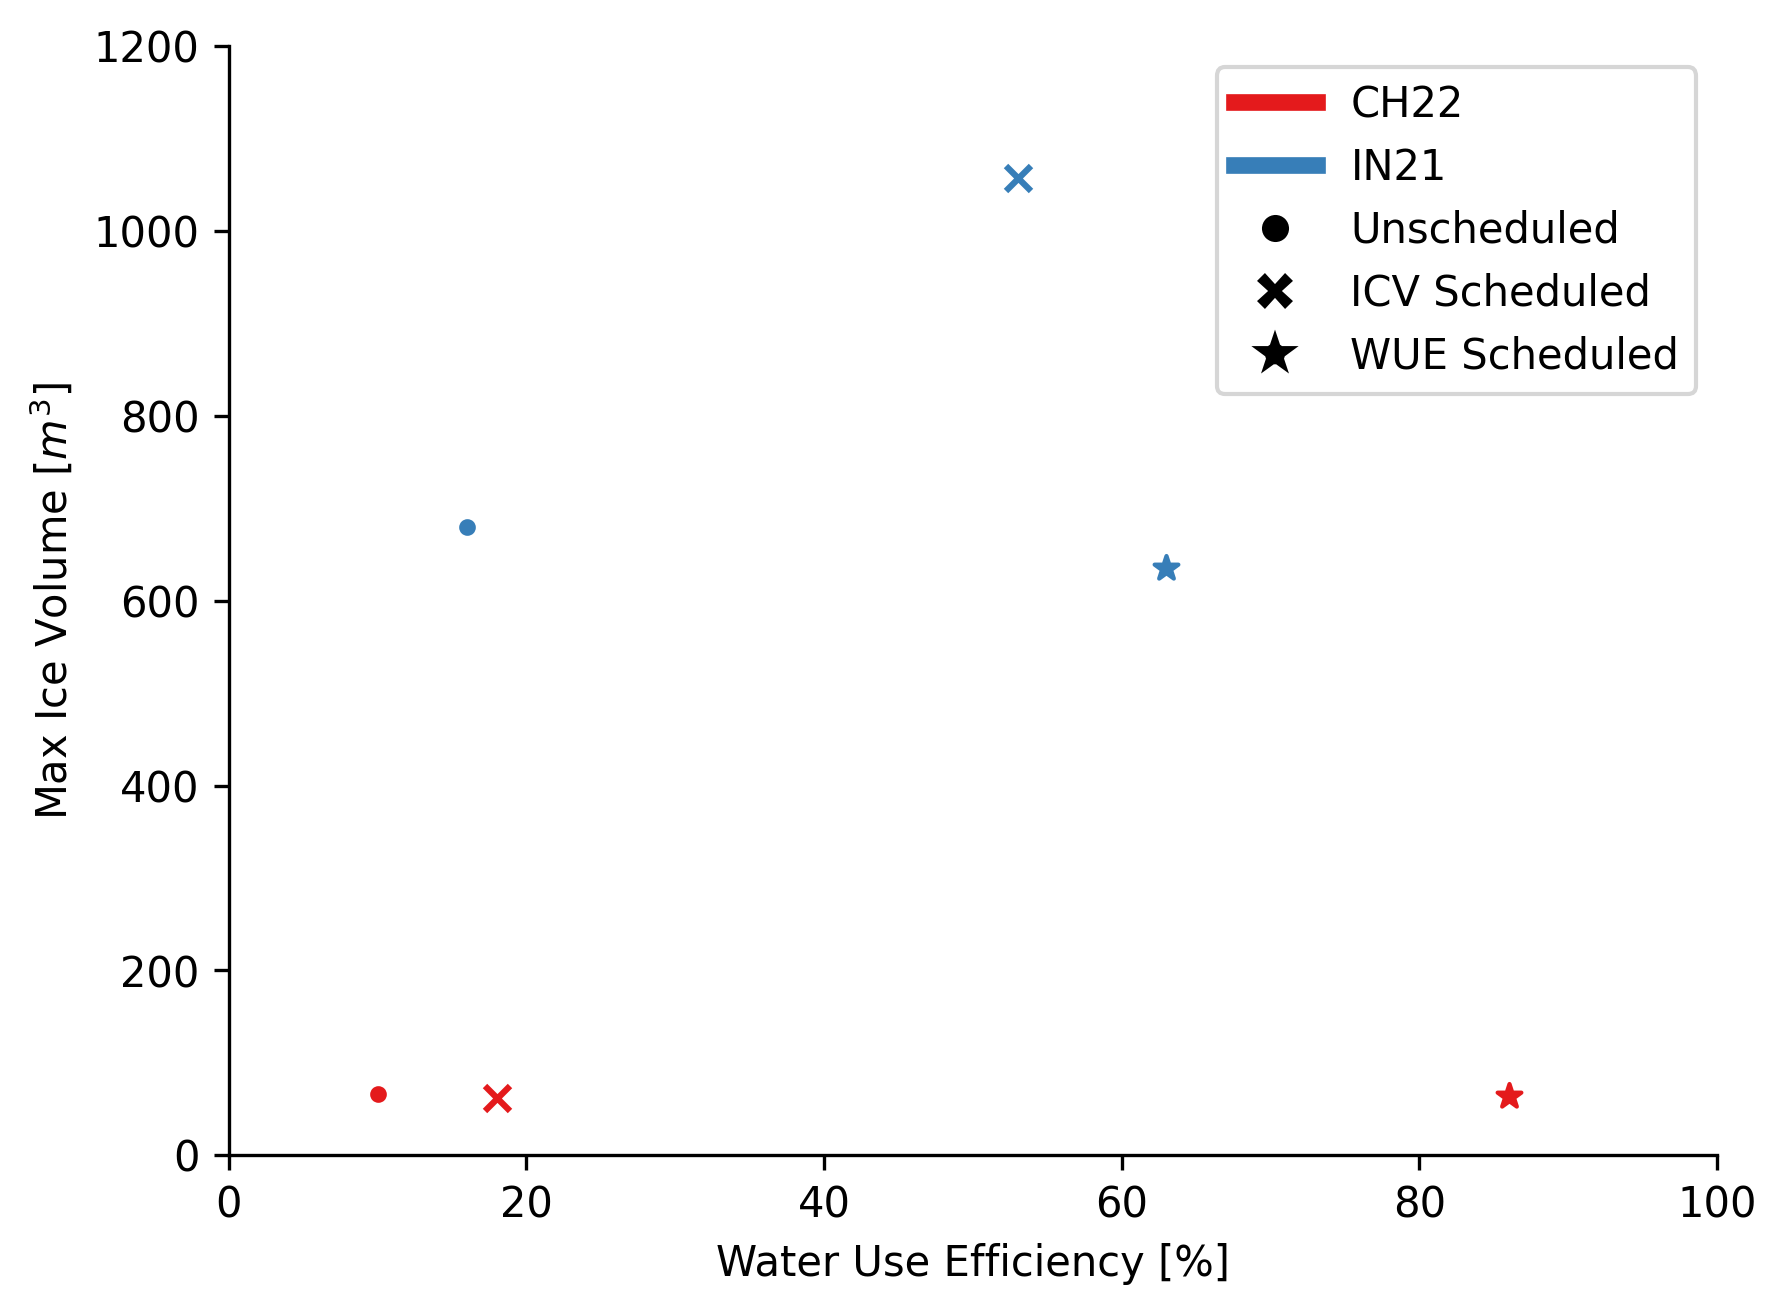
\includegraphics[width=\textwidth]{Figures/wue.png}

\caption{(a) The maximum volumes and water-use efficiency estimated for AIRs constructed in different locations
(represented by colours) with different fountain scheduling strategies (represented by symbols). Experimental
values are highlighted by circles and simulated values are highlighted by squares. (b) Comparison of
the unscheduled and scheduled fountain's discharge rates at the IN21 location.}

\label{fig:wue}
\end{figure*}

The water-use efficiency of all the unscheduled fountains are below 20 \%. In general, the water-use efficiency
increases more than three fold when the weather-sensitive or water-sensitive fountain is used in both the
locations.  

For the Indian location, the three kinds of fountains yield significantly different results.  The discharge
duration and the max discharge rate of the three IN21 fountains were responsible for these different results
(see Fig. \ref{fig:wue} (b)). The max discharge rate of the unscheduled fountain was more than twice that of
scheduled fountains resulting in a high water loss. Freezing events in the fountain pipeline caused frequent
interruptions in the unscheduled discharge rate (see Fig. \ref{fig:wue} (b)). In contrast, the mean freezing
rates of the other two fountains during these events were above their median values. This was because too cold
temperatures freezes water inside rather than outside the fountain system instigating these freezing events in
the fountain pipeline. Therefore, both the discharge duration and the mean freezing rate of the unscheduled
fountain was much lower resulting in lower ice volumes. The water-sensitive fountain underestimated the freezing
rate during the construction period and therefore produced much lower ice volumes compared to the
weather-sensitive fountain. 

For the Swiss locations, scheduled fountains yield better water-use efficiency but do not alter the maximum
volume obtained significantly. 

\subsection{Meteorological drivers of interannual volume variability}

The maximum volumes of the Swiss AIRs built during 2021-22 winter (CH22) is only half that of AIRs from the
previous winter (CH21). One would expect this difference is due to warmer temperatures during the CH22 winter.
But the median january temperature of CH22 winter was colder than the CH21 winter (see Fig. \ref{fig:CH_diffs}
(a)). Moreover, the volume growth of CH20 AIR is 6 fold that of CH22 AIR despite CH20 winter being 3 $\degree C$
warmer.

We suspect the primary driver of volume difference across different winters is instead the spray radius (see
Fig. \ref{fig:CH_diffs} (b)). However, this observation contradicts our expectation that AIRs using the same
water source and fountain designs have similar spray radius. Moreover, manual measurements of the fountain spray
radius were observed to be lesser than the drone observations of the ice radius. These two observations imply
that meteorological conditions also affect ice radius besides the engineering design of the fountain nozzle.
Particularly, wind drift of water droplets could play a major role in temporal fluctuations of the ice radius.

\begin{figure*}[t]
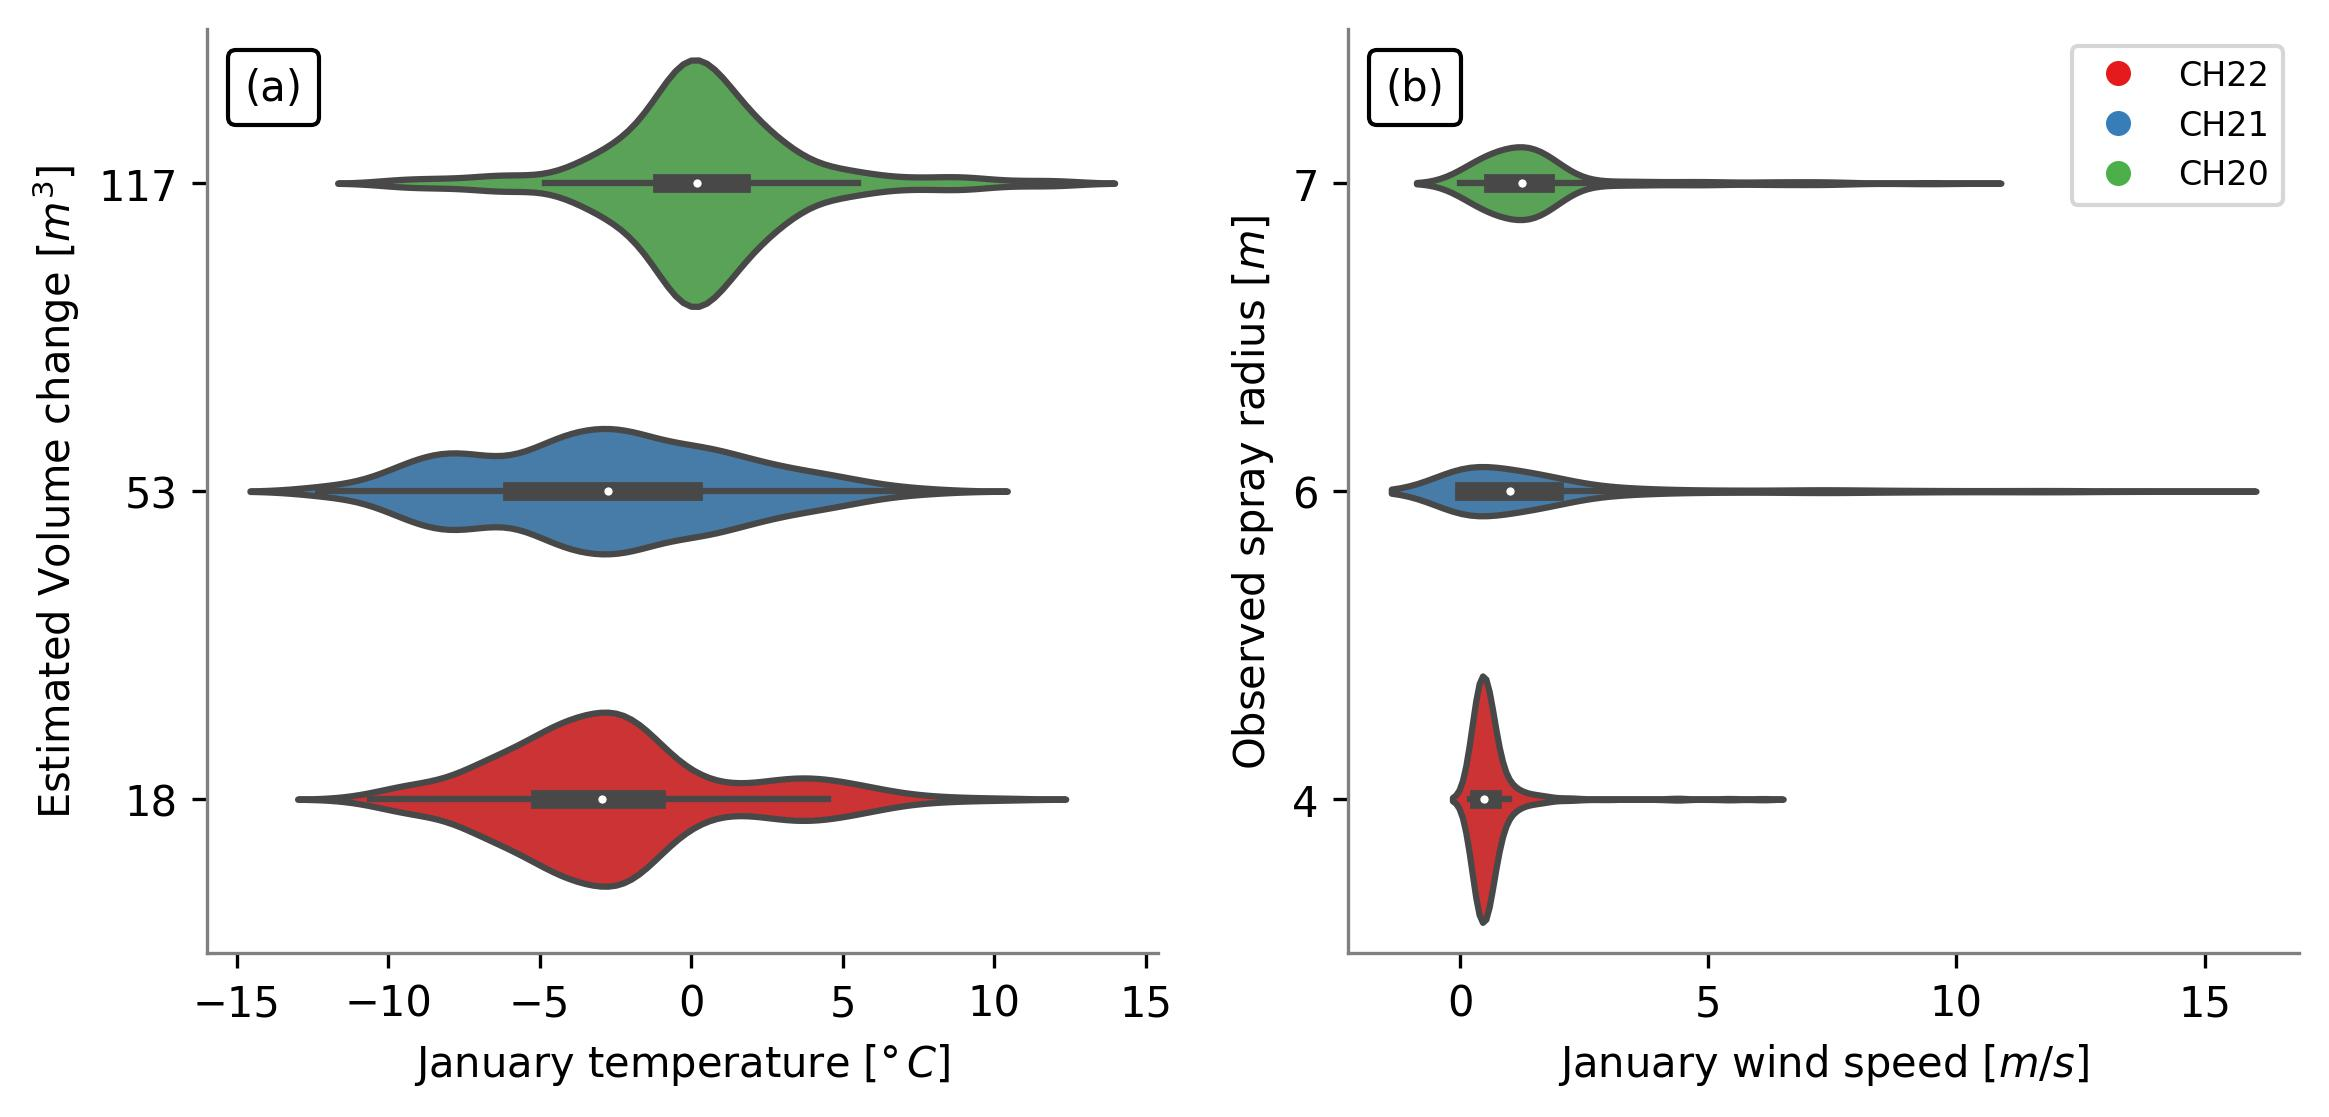
\includegraphics[width=\textwidth]{Figures/CH_diffs.jpg}

\caption{(a) Estimated volume change and median temperature and (b) Observed spray radius and median wind speed
during january for AIRs built across three winters. } 

\label{fig:CH_diffs} 
\end{figure*}

To validate this hypothesis, we model the projectile motion of scheduled fountain water droplets with wind speed
values taken from CH22 and CH21 experiments respectively. The details about the methodology used to do this is
explained in Appendix \ref{sec:r_F}. Fig. \ref{fig:wind} shows the modelled spray radius produced using these
two wind datasets and compares them with the measured spray radius values. As illustrated, wind speed drives the
temporal variation in the spray radius. Moreover, the spray radius of the scheduled fountain with CH22 wind
values is much higher than when using CH21 wind values. Therefore, the determination of the fountain spray
radius cannot be performed using the characteristics of the fountain nozzle alone since it is significantly
influenced due to the temporal variation of the wind speed.

\begin{figure*}[t]
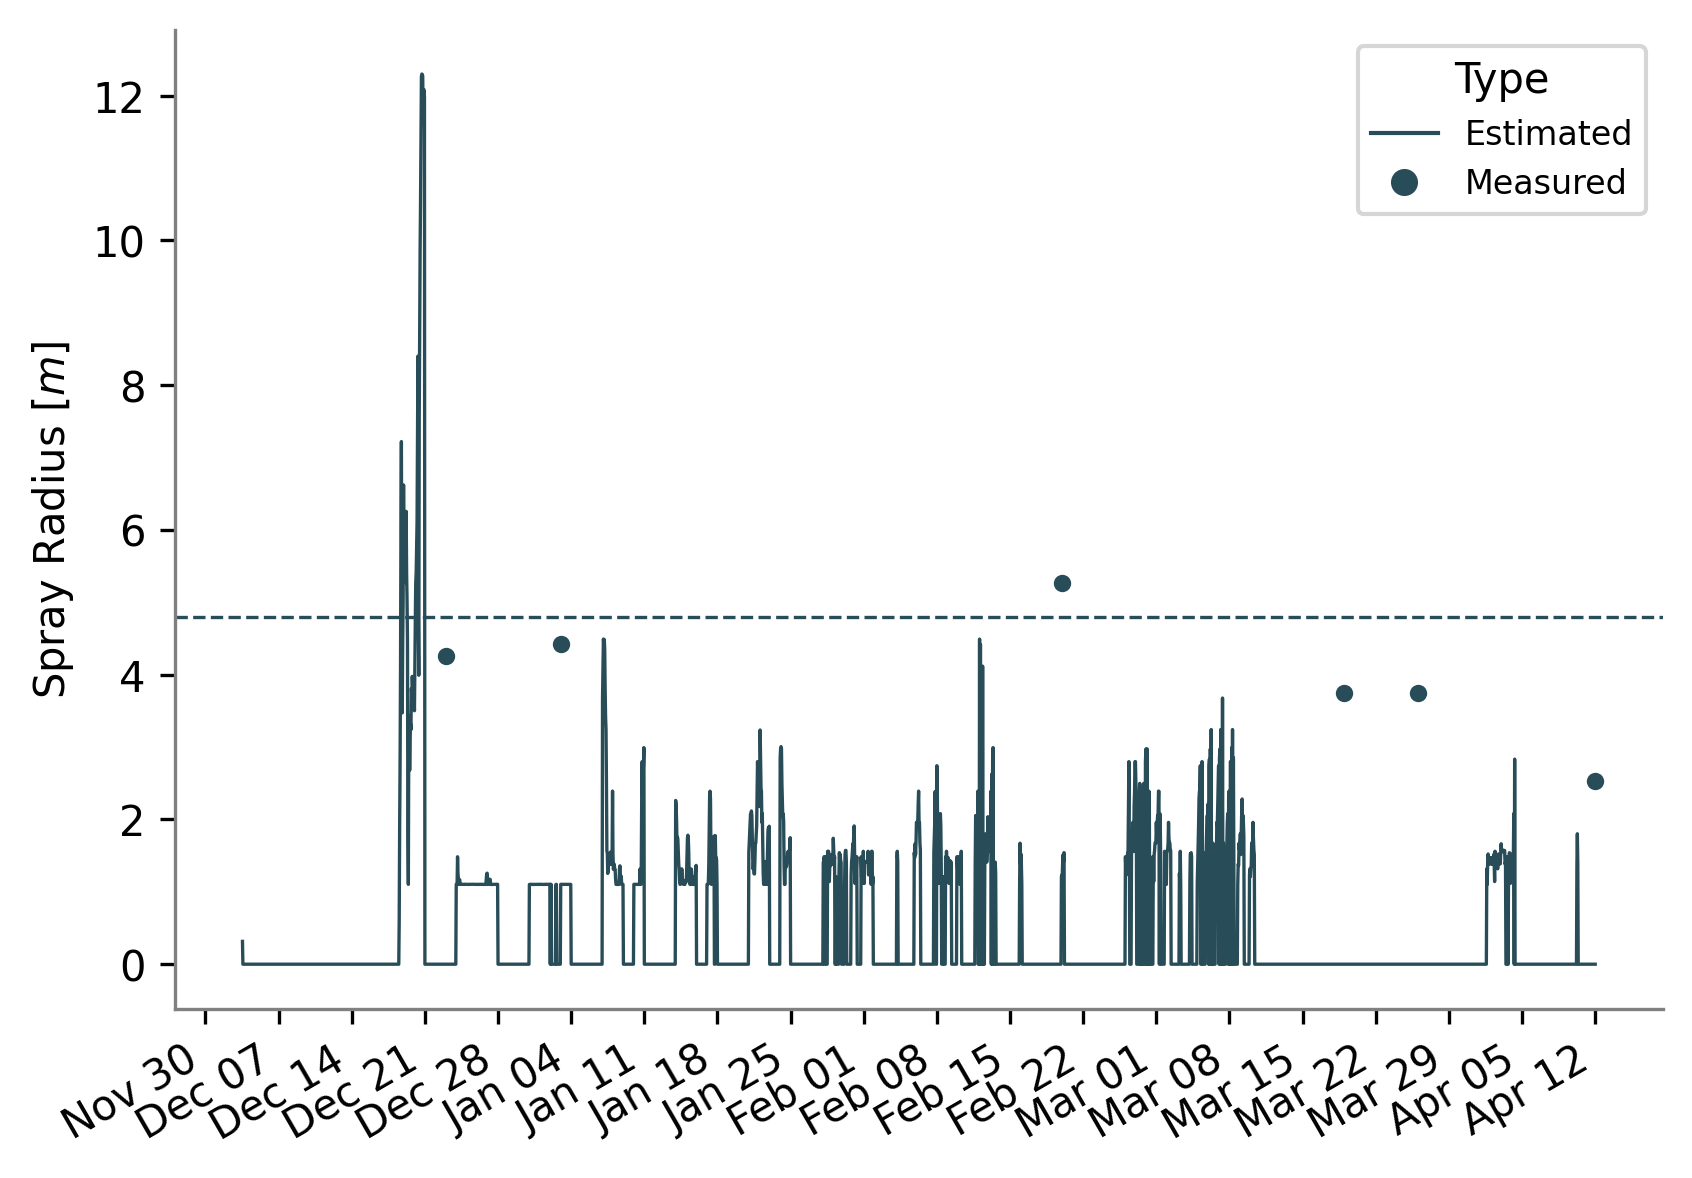
\includegraphics[width=12 cm]{Figures/radf.png}
\caption{Modelled spray radius using wind values from CH22 and CH21 experiments. Measured spray radius are
indicated as dots.}
\label{fig:wind}
\end{figure*}

\subsection{Additional water losses}

In practice, parts of the water volumes exiting the fountains do not reach the ground due to both thermodynamic
(evaporation and sublimation) and mechanical (wind-driven redistribution) effects. While these water losses can
be significant \citep{hanzerSimulationSnowManagement2020}, simulating them using physical formulations is
challenging since it is sensitive to the diameter of water droplets produced by the fountain.


\conclusions

In this paper, an automated AIR construction strategy is presented and compared with a traditional strategy
using data collected in Guttannen, Switzerland and Gangles, India.

The main purpose of this study was to quantify the influence of different fountain scheduling strategies on the
water use efficiency and volumes of AIRs exposed to identical weather conditions. We found that overwatering by
unscheduled fountains not just increased the fountain wastewater production but also enhanced the melting rate
of AIRs, mainly due to its surface albedo and fountain heat flux feedbacks. Scheduled fountains, in contrast,
consumed only 13 \% of the unscheduled fountain's water supply. However, the volume evolution of both the AIRs
showed no significant variations. 

Two different model forcings sensitive to the construction location's limited weather windows or water supply
were used to recommend two types of scheduled discharge rates favouring higher volumes and better water use
efficiencies, respectively. Nevertheless, these models were able to capture more than 44 \% of the freezing rate
variations of the traditional AIR. Simulations converting several unscheduled fountains to scheduled ones show
that atleast a three fold increase in water use efficiency is possible without compromising on meltwater
production.

Higher wind speeds drove the volume differences of AIRs constructed in the Swiss location across three
consecutive winters. The influence of wind-driven redistribution on the spray radius managed to generate AIRs
six times bigger in spite of temperatures being 3 $\degree C$ warmer. In contrast, higher wind speeds can also
cause water losses if water droplets are distributed beyond the spray radius. Therefore, a critical wind speed
needs to be determined in order to force wind-driven redistribution to increase the spray radius rather than the
water losses. Future selection of construction locations and design of automation algorithms need to capitalise
on wind-driven redistribution effects to further increase their water use efficiency.

Fountain nozzles play an important role in the construction process. First, they consume most of the input water
pressure to form water droplets. Second, their engineering design determines the droplet size distribution and
spray radius. Future research, therefore, must be devoted to engineer fountain nozzles that create water
droplets with a size distribution that requires lesser energy consumption and a trajectory that increases their
spray radius.

\appendix


\section{Model forcing based on water-use efficiency and maximum volume objectives} \label{sec:SEB}

The model complexity and data requirement \citep{balasubramanianInfluenceMeteorologicalConditions2022} were
reduced through assumptions that optimise for the ice volume or the water-use efficiency objectives. The
corresponding model assumptions are called IVOM and WEOM respectively. We define the freezing rate and melting
rate as the positive and negative mass change rate, respectively. Assumptions are chosen, based on whether they
overestimate/underestimate the freezing rate. IVOM assumptions overestimates freezing rate whereas WEOM
assumptions underestimates freezing rate. We describe these two kinds of assumptions applied on each of the
energy balance components below: 

\subsection{Surface Area $A_{cone}$ assumptions}

Determination of the surface area during the accumulation period is achieved by assuming a constant ice cone
radius equal to the fountain spray radius. The surface area scales the freezing rate of the AIR. Hence, for the
IVOM version, we assume the maximum possible slope of 1 for the ice cone or in other words $h_{cone} = r_{F}$.
Therefore, area is estimated as:  

\begin{equation} A_{cone} =\sqrt{2} \cdot \pi \cdot r_{F}^2  \end{equation}

Similarly, for the water-use efficiency objective, the area of the conical AIR is approximated to the area of
its circular base. Therefore, area is estimated as:

\begin{equation} A_{cone} =\pi \cdot r_{F}^2  \end{equation}

\subsection{Net shortwave radiation \texorpdfstring{$q_{SW}$}{Lg} assumptions}
\label{sec:SW}

The net shortwave radiation $q_{SW}$ is computed as follows:

\begin{equation} 
q_{SW} = (1- \alpha) \cdot ( SW_{direct} \cdot f_{cone} + SW_{diffuse})
\label{eqn:SW} 
\end{equation}

where $\alpha$ is the albedo value ; $SW_{direct}$ is the direct shortwave radiation; $SW_{diffuse}$ is the
diffuse shortwave radiation and $f_{cone}$ is the solar area fraction.

The data requirement was reduced by estimating the global shortwave radiation and pressure directly using the
location's coordinates and altitude through the solar radiation model described in
\citet{holmgrenPvlibPythonPython2018}. The algorithm used to estimate the clear-sky global radiation is
described in \citet{ineichenBroadbandSimplifiedVersion2008}.  

The diffuse and direct shortwave radiation is determined using the estimated global solar radiation as follows:

\begin{equation}
\begin{split}
  SW_{diffuse} &= cld \cdot SW_{global}\\
  SW_{direct} &= (1-cld) \cdot SW_{global}
\end{split}
\end{equation}

where $cld$ is the cloudiness factor. $cld$ is assumed to be 1 and 0 for the water-use efficiency and ice volume
objective respectively.

We ignore the variations in the albedo and assume it to be equal to snow albedo and ice albedo for the  ice
volume and water-use efficiency objective, respectively.

The solar area fraction $f_{cone}$ of the ice structure exposed to the direct shortwave radiation depends on the
shape considered. It is computed as

\begin{equation}
		f_{cone} =\frac{(0.5 \cdot r_{cone} \cdot h_{cone}) \cdot cos \theta_{sun} +(\pi \cdot
			{(r_{cone})}^2/2) \cdot sin \theta_{sun} }{\pi \cdot r_{cone} \cdot ({(r_{cone})}^2+{(h_{cone})}^2)^{1/2}}\\
\end{equation}

For the ice volume objective, since we assume the slope of the cone to be 1, $f_{cone}$ is determined as follows:

\begin{equation}
		f_{cone} =\frac{ cos \theta_{sun} + \pi \cdot sin \theta_{sun} }{2\sqrt{2} \cdot \pi }
\end{equation}

Similarly, for the water-use efficiency objective, since we assume the slope of the cone to be negligible, we get:

\begin{equation}
		f_{cone} =\frac{ sin \theta_{sun} }{2 }
\end{equation}

\subsection{Net Longwave radiation \texorpdfstring{$q_{LW}$}{Lg} assumptions} 

We assume $T_{ice} = 0 \degree C$ in order to determine outgoing longwave radiation. Since it is challenging to
constrain the minimum ice temperature, we maintain this assumption for both our objectives. However, in order to
estimate atmospheric emissivity, we again assume $cld$ to be 1 and 0 for the water-use efficiency and ice volume
objective respectively.

\subsection{Turbulent fluxes assumptions} \label{sec:Qs}

Turbulent fluxes estimation depend on the slope of the cone through the $\mu_{cone}$ parameter. As suggested 
by \citet{oerlemansBriefCommunicationGrowth2021}, we estimated this parameter as follows:

\begin{equation}
  \mu_{cone} =1 + s_{cone}/2
\end{equation}

Hence, the $\mu_{cone}$ parameter takes values of 1.5 and 1 for the ice volume and water-use efficiency
objective respectively.  Since turbulent fluxes impact both the freezing and the melting rates, this assumption
may not favor the corresponding objectives for certain sites.

\appendixtables   %% needs to be added in front of appendix tables

\begin{table}
  \caption{Free parameters in the model categorised as constant, model hyperparameters and weather 
  parameters with their respective values/ranges.}

	\label{tab:parameters}
	\begin{tabular}{lllll}
		\toprule

		\textbf{Constant Parameters}                       & \textbf{Symbol} & \textbf{Value} &
    \textbf{Unit} & \textbf{References} \\
    Van Karman constant & $\kappa$      & 0.4        &dimensionless & \citet{cuffeyPhysicsGlaciers2010}              \\
    Stefan Boltzmann constant & $\sigma$ & $\num{5.67 e-8} $& $W\, m^{-2}\, K^{-4}$ & \citet{cuffeyPhysicsGlaciers2010}\\
    Air pressure at sea level & $p_{0,a}$ & 1013 & $hPa$  & \citet{molgAblationAssociatedEnergy2004}\\
    Density of water & $\rho_{w}$ & 1000 & $kg\, m^{-3}$    & \citet{cuffeyPhysicsGlaciers2010}\\
    Density of ice & $\rho_{ice}$ & 917 & $kg\, m^{-3}$ & \citet{cuffeyPhysicsGlaciers2010}\\
    Density of air & $\rho_{a}$ &  1.29 & $kg\, m^{-3}$   & \citet{molgAblationAssociatedEnergy2004}\\
    Specific heat of water & $c_{w}$ & 4186 & $J\, kg^{-1}\,\degree C^{-1}$  & \citet{cuffeyPhysicsGlaciers2010}\\
    Specific heat of ice & $c_{ice}$ & 2097 & $J\, kg^{-1}\,\degree C^{-1}$ & \citet{cuffeyPhysicsGlaciers2010}\\
    Specific heat of air & $c_{a}$ & 1010 & $J\, kg^{-1}\,\degree C^{-1}$ & \citet{molgAblationAssociatedEnergy2004}\\
    Thermal conductivity of ice & $k_{ice}$ & 2.123  & $W\, m^{-1}\, K^{-1}$ & \citet{bonalesThermalConductivityIce2017} \\
    Latent Heat of Sublimation & $L_{s}$ & \num{2.848e6}  & $J\, kg^{-1}$ &   \citet{cuffeyPhysicsGlaciers2010}\\
    Latent Heat of Fusion & $L_{f}$ & \num{3.34e5} & $J\, kg^{-1}$ & \citet{cuffeyPhysicsGlaciers2010}\\
    Gravitational acceleration & $g$ & 9.81 & $m\, s^{-2}$ &\citet{cuffeyPhysicsGlaciers2010}\\
    Weather station height & $h_{AWS}$ & 2 & $m$ & assumed \\
    Model timestep                            & $\Delta t$            & $3600$           & $s$ & assumed \\\midrule

		\textbf{Model Hyperparameters} & \textbf{Symbol} & \textbf{Range} & \textbf{Unit} & \textbf{References} \\
    Surface layer thickness             & $\Delta x$            & $[\num{1e-2},\num{1e-1}]$           & $m$ & assumed
    \\\midrule
		\textbf{Weather Parameters} & \textbf{Symbol} & \textbf{Range} & \textbf{Unit} & \textbf{References} \\
    Ice Emissivity                      & $\epsilon_{ice}$      & $[0.95,0.99]$         & dimensionless & \citet{horiInsituMeasuredSpectral2006}             \\
    Surface Roughness                   & $z_0$                 & $[\num{1e-3},\num{5e-3}]$            & $m$  & \citet{brockMeasurementParameterizationAerodynamic2006}       \\
    Ice Albedo                          & $\alpha_{ice}$        & $[0.15,0.35]$         & dimensionless  &
    \citet{steinerModellingIcecliffBackwasting2015};            \\
    & &    &  & \citet{zollesRobustUncertaintyAssessment2019}      \\
    Snow Albedo                         & $\alpha_{snow}$       & $[0.8,0.9]$        & dimensionless  & \citet{zollesRobustUncertaintyAssessment2019}              \\
    Precipitation Temperature threshold & $T_{ppt}$             & $[0,2]$            & $\degree C$& \citet{shichangResponseZhadangGlacier2010}  \\
    Albedo Decay Rate                   & $\tau$                & $[10,22]$           & $days$ &
    \citet{schmidtImportanceAccurateGlacier2017};      \\
    & &    &  & \citet{oerlemansYearRecordGlobal1998}      \\\midrule
	\end{tabular}
\end{table}
\clearpage

\section{Modelling fountain spray radius} \label{sec:r_F}

The fountain spray radius is defined as the largest horizontal distance covered by fountain water droplets. This
can be determined by modelling the trajectory of these droplets using the projectile motion equation. This
projectile motion starts at the fountain nozzle and ends at the AIR surface.  To obtain the droplet speeds, we
use the the measured aperture diameter ($dia = 10 mm$) and discharge rate of the scheduled fountain  through the
following equation:

\begin{equation}
	\label{eqn:dis}
 v = 4 \cdot Q/(\pi \cdot dia^2)
\end{equation}

To obtain the spray radius, we use the optimum launch angle $\theta = 45 \degree$ in the projectile motion
equation to get:

\begin{equation}
  \label{eqn:radf}
  r = \frac{v \cdot(v + \sqrt{v^2 + 4hg)}}{2g}
\end{equation}

The influence of wind is included in the spray radius by multiplying the wind speed with the time of flight of
the water droplets.

\noappendix 

\authorcontribution{
  Suryanarayanan Balasubramanian: Conceptualization, Methodology, Investigation, Data curation, Visualization, Software,
Writing- Original draft preparation

  Martin Hoelzle: Conceptualization, Supervision, Investigation, Writing- Reviewing and Editing 

  Roger Waser: Resources- Automation system, Writing- Reviewing and Editing.} %% this section is mandatory

\competinginterests{The authors declare that they have no known competing financial interests or personal
relationships that could have appeared to influence the work reported in this paper.} %% this section is mandatory even if you declare that no competing interests are present

\begin{acknowledgements}
TEXT
\end{acknowledgements}

\bibliographystyle{copernicus}
\bibliography{zot_refs.bib}

\end{document}
